\documentclass[12pt, a4paper]{article}
\usepackage{comment}
\usepackage{ragged2e}
\usepackage{amsmath}
\usepackage{xcolor}
\usepackage{multirow}
\usepackage{caption}
\usepackage{tikz}
\usepackage{booktabs}
\usepackage{tabu}
\usepackage{placeins}
\usepackage{pdflscape}
\usetikzlibrary{arrows}
\usepackage{hyperref}
\usepackage{multirow}
\usepackage{subcaption}


\captionsetup{font=footnotesize,labelfont=footnotesize}

\hypersetup{
    colorlinks=true,
    linkcolor=blue,
    filecolor=blue,      
    urlcolor=blue,
    citecolor=blue
}

\usepackage{natbib}
\usepackage[title]{appendix}

\tikzstyle{startstop} = [rectangle, rounded corners, minimum width=2cm, minimum height=0.75cm,text centered, draw=black, fill=red!30]

\tikzstyle{startstop1} = [rectangle, rounded corners, minimum width=2cm, minimum height=0.75cm,text centered, draw=black, fill=blue!30]

\tikzstyle{startstop2} = [rectangle, rounded corners, minimum width=2cm, minimum height=0.75cm,text centered, draw=black, fill=yellow!30]

\tikzstyle{startstop3} = [rectangle , rounded corners, minimum width=0.5cm, minimum height=0.75cm,text centered,draw=black]


\tikzstyle{io} = [trapezium, trapezium left angle=70, trapezium right angle=110, minimum width=2cm, minimum height=0.75cm, text centered, draw=black, fill=blue!30]



\tikzstyle{process} = [rectangle, minimum width=2cm, minimum height=1cm, text centered, draw=black, fill=green!30]

\tikzstyle{decision} = [diamond, minimum width=0.75cm, minimum height=0.75cm, text centered, draw=black, fill=green!30]

\tikzstyle{arrow} = [thick,->,>=stealth]



\def\sym#1{\ifmmode^{#1}\else\(^{#1}\)\fi}


\renewcommand{\today}{\ifcase \month \or January\or February\or March\or %
April\or May \or June\or July\or August\or September\or October\or November\or %
December\fi, \number \year} 

\title{Connected Stocks: Evidence from Tehran Stock Exchange}
%\subtitle{}
\author{S.M. Aghajanzadeh\sym{*} \qquad M. Heidari\sym{*} \qquad M. Mohseni\sym{*} \\
\sym{*} \footnotesize  Tehran Institute for Advanced Studies, Khatam University, Tehran, Iran
}

\def\boxit#1{%
  \smash{\color{red}\fboxrule=1pt\relax\fboxsep=2pt\relax%
  \llap{\rlap{\fbox{\vphantom{0}\makebox[#1]{}}}~}}\ignorespaces
}







\begin{document}
\maketitle


\begin{abstract}
We connect stocks by their common blockholders. We introduce a measure that captures the extent to which distribution of joint holders. A vital feature of the measure is allowing the joint ownership distributions to affect the measure. After that, We show that the degree of shared ownership that crosses a threshold forecasts return correlation, controlling for exposure to systematic return factors and other pair characteristics. We study this effect in business groups and find that being in the same business group significantly affects comovement. Further investigations explain that comovement increases when a bank is a business group's ultimate owner.
\end{abstract}

\textit{Keywords:} Asset management; Institutional investors; Return comovement; common
Ownership; Indexing 
\\

\textit{JEL Classifications:} G10; G11; G23 



\section{Introduction}


\FloatBarrier



\section{Measurement of cross-ownership}


In table \ref{maasurmentsSummary} we summarize common ownership measurements which are used in literature. There are two groups of measurement for common ownership.
First of all, model-based measures that capture common ownership base on a proper  model. These measures have a better economic interpretation, but most of them are bi-directional or industry-level measures.(e.g, \cite{harford2011institutional}; \cite{azar2018anticompetitive}; \cite{gilje2020s})

 In addition to model-based measures, some ad hoc common ownership measures are used in the empirical literature. There is significant doubt on how these measures capture common ownership's impact on the management, and many of them have unappealing properties.(e.g, \cite{AntonPolk}; \cite{azar2011new}; \cite{freeman2019effects}; \cite{hansen1996externalities};  \cite{he2017product}; \cite{he2019internalizing}; \cite{lewellen2021does}; \cite{newham2018common})


\begin{table}[htbp]
\centering
\scriptsize
\caption{ This table summarizes common ownership measurements in the literature.}
\label{maasurmentsSummary}
\resizebox{\textwidth}{!}{
    \begin{tabular}{cllc}
    \hline\hline
    \multicolumn{1}{c}{Group}      & \multicolumn{1}{c}{Paper} & \multicolumn{1}{c}{measurment} & \multicolumn{1}{c}{Flaws} \\
          \hline\hline
           \addlinespace
    \multicolumn{1}{c}{\multirow{5}[2]{*}{Model Based}} &  \cite{harford2011institutional}     &  \scriptsize  $
       \sum_{i\in I^{A,B}}\frac{\alpha_{i,B}}{\alpha_{i,A} + \alpha_{i,B}}     $     & Bi-directional \\
      \addlinespace 
          &  \cite{azar2018anticompetitive}     &  $   \sum_{j} \sum_k s_j s_k \frac{\sum_i \mu_{ij} \nu_{ik}}{\sum_i \mu_{ij} \nu_{ij}}   $     & Industry level \\
          \addlinespace
          &  \cite{gilje2020s}     &    $ \sum_{i = 1}^{I} \alpha_{i,A}g(\beta_{i,A})\alpha_{i,B}    $   & Bi-directional  \\
          \midrule
    \addlinespace 
    \multicolumn{1}{c}{\multirow{7}[5]{*}{Ad hoc}} & \cite{he2017product};      &  \multirow{2}{*}{$ \sum_{i\in I^{A,B}} 1 $}     & invariant to the level   \\
          & \cite{he2019internalizing} & & of ‌common ownership \\
          \addlinespace
          &  \cite{newham2018common}     &   $ \sum_{i\in I^{A,B}} min\{\alpha_{i,A},\alpha_{i,B}\} $    & ? \\
          \addlinespace
          & \multirow{2}{*}{   \cite{AntonPolk} }  &  \multirow{2}{*}{ $ \sum_{i\in I^{A,B}} \alpha_{i,A}\frac{\bar{\nu}_A}{\bar{\nu}_A +\bar{\nu}_B } + \alpha_{i,B}\frac{\bar{\nu}_B}{\bar{\nu}_A +\bar{\nu}_B }  $ }   &  Invariant to the  \\
           & & & decomposition of ownership \\
          \addlinespace
          & \cite{freeman2019effects}; & \multirow{2}{*}{ $ \sum_{i\in I^{A,B}} \alpha_{i,A} \times \sum_{i\in I^{A,B}} \alpha_{i,B} $ }&?\\
                    &  \cite{hansen1996externalities} & & ?\\
                    \hline\hline
    \end{tabular}
    }
\end{table}



In our primary analysis, we estimate the impact of common ownership on pair's correlation. For this purpose, we need a pair-level measure with a good economic interpretation that is not bi-directional. As a result, we propose a modification for Anton's measure (\cite{AntonPolk}) that captures the extent of common ownership distribution and apply this measure in this study.

\subsection{Modified Anton's measure }
We reformulate mentioned Anton's measure in table \ref{maasurmentsSummary}. This factor measure common ownership as the total value of
stock held by the F common-holders of the two stocks, scaled by the total market capitalization of the two stocks
\begin{equation}
\text{Overlap}_{Sum}(i, j) = \frac{\sum_{f = 1}^{F} (S^f_{i,t}P_{i,t}+S^f_{j,t}P_{j,t})}{S_{i,t}P{i,t} + S_{j,t}P{j,t}}
\label{Sum}
\end{equation}
 where $ S^f_{i,t}$ is the number of shares held by owner f
at time t trading at price $ P{i,t} $ with total shares outstanding of $ S_{i,t} $, and similarly for stock j. 
As shown in equation \ref{Sum}, this measure neglects different distribution of common owners and represents the percent of joint-held market capitalization from the total market capitalization of the two stocks.

We reweight this formula to capture the difference between ownership distribution. Our proposed measures are shown in equation \ref{sqrt} and \ref{Quadratic} where all variables as the same Anton's measure. Both modified measures represent the number of equal percents held block-holder. In other words, If for a pair of stocks with n mutual owners, all owners have even shares of each firm's market cap, then the proposed indexes will be equal to number of holders.\footnote{ \tiny
\begin{itemize}
\item Each holder owns $ 1/n $ of each firm ,Firm's market cap is $ \alpha_1 $ and $ \alpha_2 $, So for each holder of firms we have $ S^f_{i,t}P_{i,t} = \alpha_i/n $\\
 $
[  \frac{\sum_{f=1}^{n} \sqrt{\alpha_1/n}+\sum_{f=1}^{n} \sqrt{\alpha_2/n}}{\sqrt{\alpha_1} + \sqrt{\alpha_2}}]^2 
= [\frac{\sqrt{n}(\sqrt{\alpha_1} +\sqrt{\alpha_2 })}{\sqrt{\alpha_1} + \sqrt{\alpha_2}}]^2 = n $
\\
$
[\frac{\sum_{f=1}^{n} {(\alpha_1/n)^2}+\sum_{f=1}^{n} {(\alpha_2/n)^2}}{\alpha_1^2 +{\alpha_2}^2}]^{-1} = [\frac{{\alpha_1^2 + \alpha_2^2 }}{n(\alpha_1^2 + \alpha_2^2)}]^{-1} = n
$
\end{itemize}}



\begin{equation}
       \text{Overlap}_{Sqrt}(i, j) =  [\frac{\sum_{f =1}^{F}(\sqrt{S^f_{i,t}P_{i,t}}+\sqrt{S^f_{j,t}P_{j,t}})}{\sqrt{S_{i,t}P{i,t}} + \sqrt{S_{j,t}P{j,t}}}]^2 
            \label{sqrt}
\end{equation}

\begin{equation}
\text{Overlap}_{Quadratic}(i, j) =  [{\frac{\sum_{f = 1}^{F}[(S^f_{i,t}P_{i,t})^2+(S^f_{j,t}P_{j,t})^2]}{(S_{i,t}P{i,t})^2 + (S_{j,t}P{j,t})^2}}]^{-1}
\label{Quadratic}
\end{equation}

There are some numeric examples for better comparison. Two firms (X and Y) have one common owner who has $ \alpha $ and $ \beta $ from each market capitalization, respectively. (illustrated in figure \ref{gExample1}) 
for better illustration, assume that the sum of holder's ownership equal to 100 percent ($ \alpha + \beta  = 100$), and two firms' market cap is equal. 


\begin{figure}[htbp]
\centering
\caption{ Numeric example 1 }
\label{gExample1}
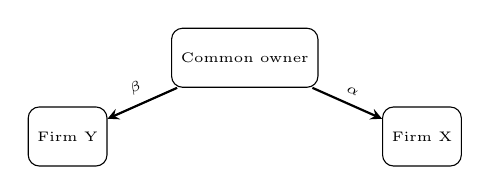
\begin{tikzpicture}[node distance=1cm]

\node (Firm) [startstop3] {\tiny Firm X};
\node (Firm2) [startstop3,right of = Firm  , xshift=-5.5cm ] {\tiny Firm Y};
\node (Owner) [startstop3,right of = Firm , yshift=1cm , xshift=-3.25cm ] {\tiny Common owner };


\draw[arrow] (Owner) -- node[sloped, anchor=center, above] {\tiny $ \alpha $} (Firm) ;

\draw[arrow] (Owner) -- node[sloped, anchor=center, above] {\tiny $ \beta $} (Firm2) ;
%
%\node() at (3,0)
%    {$ \alpha + \beta = 100 $}; 
\end{tikzpicture}
\end{figure}\bigskip



We  calculate common ownership measures base on equations \ref{Sum} (Sum), \ref{sqrt} (SQRT), and \ref{Quadratic} (Quadratic) for different ownership distributions.  Figure \ref{example1Results}  reports calculations results. As we expected, Anton's measure is constant at a fixed level of aggregate common ownership, but SQRT and  Quadratic vary from concentrated to dispersed ownership.  Concentrated ownership (50-50) has a greater common ownership measure than dispersed (10-90).

\begin{figure}[htbp]
  \caption{ Comparison of three measure for common ownership}
  \label{example1Results}
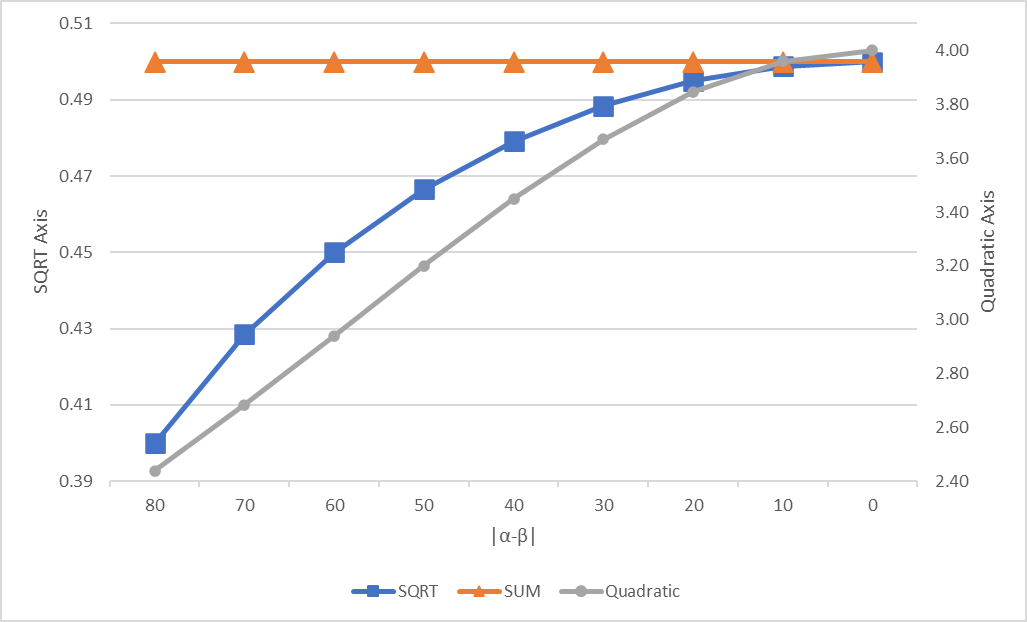
\includegraphics[width=0.47\linewidth]{1.png}
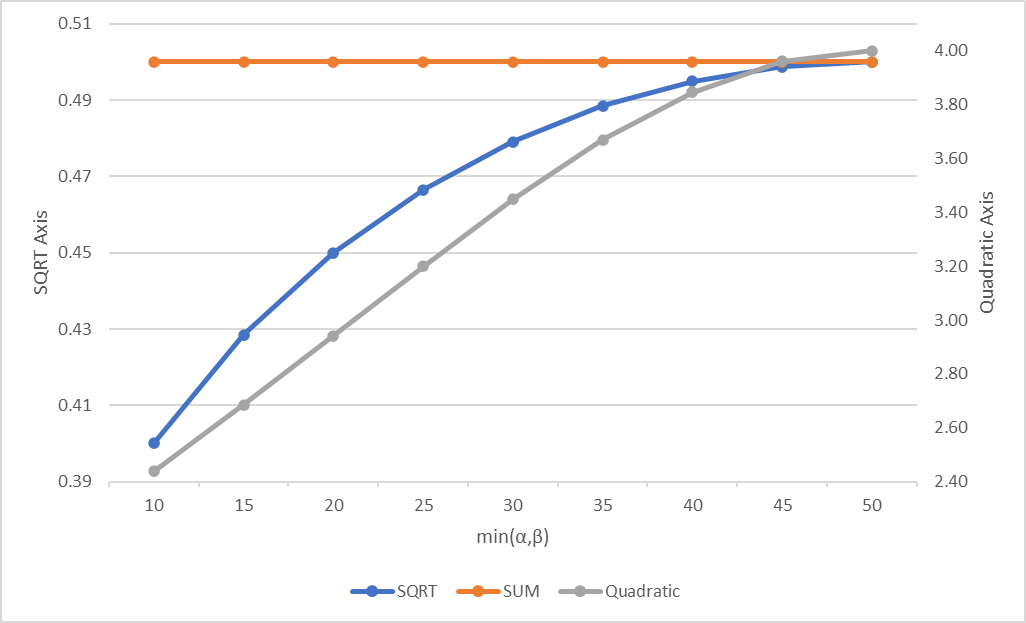
\includegraphics[width=0.47\linewidth]{2.png}

\end{figure}


Now assume that there are three common owners for the two mentioned firms. First holder's ownership from firm X and Y are respectively $\alpha_1$ and $\beta_1$. It is similar for other holders. (illustrated in figure \ref{gExample2}). As before, the firm's market cap is equal. We calculate measures for concentrated or disparate ownership and ownerships that are less than the aggregate of the firm's market cap. Table \ref{Example2} reports calculation results. For ownerships that consist of total market cap,  results are consistent with the first example. Although, when aggregate ownership decreases, the Quadratic measure denotes unrealistic numbers. We conclude that our Quadratic measure is not a good measure for common ownership.


\begin{figure}[htbp]  \centering
  \caption{ Numeric example 2}
  \label{gExample2}
  
\centering

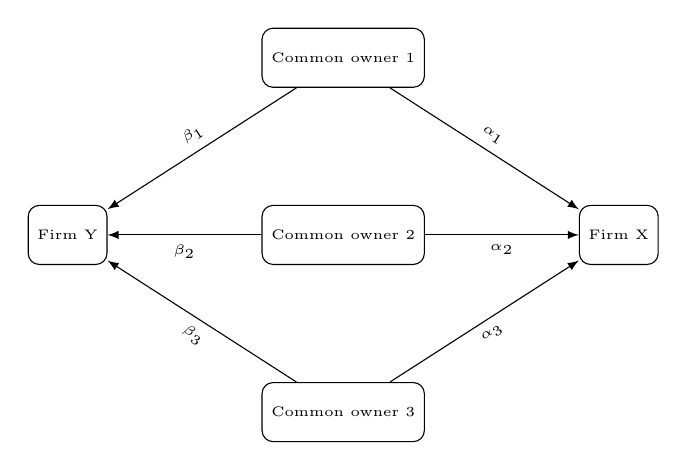
\begin{tikzpicture}[node distance=1cm]


\node (Firm) [startstop3] {\tiny Firm X};
\node (Firm2) [startstop3,right of = Firm , yshift=0cm , xshift=-8cm ] {\tiny Firm Y};

\node (Owner) [startstop3,above of = Firm , yshift=1.25cm , xshift=-3.5cm ] {\tiny Common owner 1 };


\node (Owner2) [startstop3,right of = Firm , yshift= 0 , xshift=-4.5cm ] {\tiny Common owner 2 };

\node (Owner3) [startstop3,below of = Firm , yshift=-1.25cm , xshift=-3.5cm ] {\tiny Common owner 3 };





\draw [-latex] (Owner) to [bend right =0]  node[sloped, anchor=center, above] {\tiny $ \beta_1 $} (Firm2);

\draw [-latex] (Owner) to [bend left =0]  node[sloped, anchor=center, above] {\tiny $ \alpha_1 $} (Firm);



\draw [-latex] (Owner2) to [bend right =0]  node[sloped, anchor=center, below] {\tiny $ \beta_2 $} (Firm2);

\draw [-latex] (Owner2) to [bend left =0]  node[sloped, anchor=center, below] {\tiny $ \alpha_2 $} (Firm);



\draw [-latex] (Owner3) to [bend left =0]  node[sloped, anchor=center, below] {\tiny$ \beta_3 $} (Firm2);

\draw [-latex] (Owner3) to [bend right =0]  node[sloped, anchor=center, below] {\tiny $ \alpha_3 $} (Firm);



\end{tikzpicture}

\end{figure}


\begin{table}[htbp]
\centering

\caption{ text}
\label{Example2}
 \resizebox{1\textwidth}{!}
          {
    \begin{tabular}{cccccccc}
    \hline\hline
        Ownership  & Type I & Type II & Type III & Type IV & Type V & Type VI & Type VII \\
          \hline
    $ \alpha_1 $    & 1/3 &20      &  10   & 20    & 10    & 5     & 1  \\
    $ \beta_1 $    & 1/3  & 10    & 10   & 20    & 10    & 5     & 1  \\
    $ \alpha_2 $    & 1/3  & 10    & 80    & 20    & 10    & 5     & 1 \\
    $ \beta_2 $    & 1/3  & 20    & 80    & 20    & 10    & 5     & 1  \\
    $ \alpha_3 $    & 1/3  & 70    & 10    & 20    & 10    & 5     & 1 \\
    $ \beta_3 $    & 1/3  & 70    & 10   & 20    & 10    & 5     & 1  \\
    \hline
    SQRT  & 3     &  2.56  & 2.33 & 1.8   & 0.9   & 0.45  & 0.09 \\
    SUM   & 1     & 1     & 1     & 0.6   & 0.3   & 0.15  & 0.03 \\
    Quadratic & 3     & 1.85  & 1.52  & 8.33  & 33.33 & 133.33 & 3333.33 \\
 
    \hline\hline
    \end{tabular}%
    }
\end{table}




A fundamental assumption in previous examples is equality of firms' market cap. In the last example, we relax this assumption. Table \ref{marketcap} reports calculated measures for fixed aggregate ownership on different relative market cap ratios. We extend our analysis to higher market cap ratios and report our results in figure \ref{sqrtMarket} and \ref{sumMarket}. In this setting, the SQRT measure has a better variation relative to Anton's measure. 






\begin{figure}[htbp]
\centering
 \caption{ SQRT measure for fixed aggregate ownership on different relative market cap ratios}
  \label{sqrtMarket}
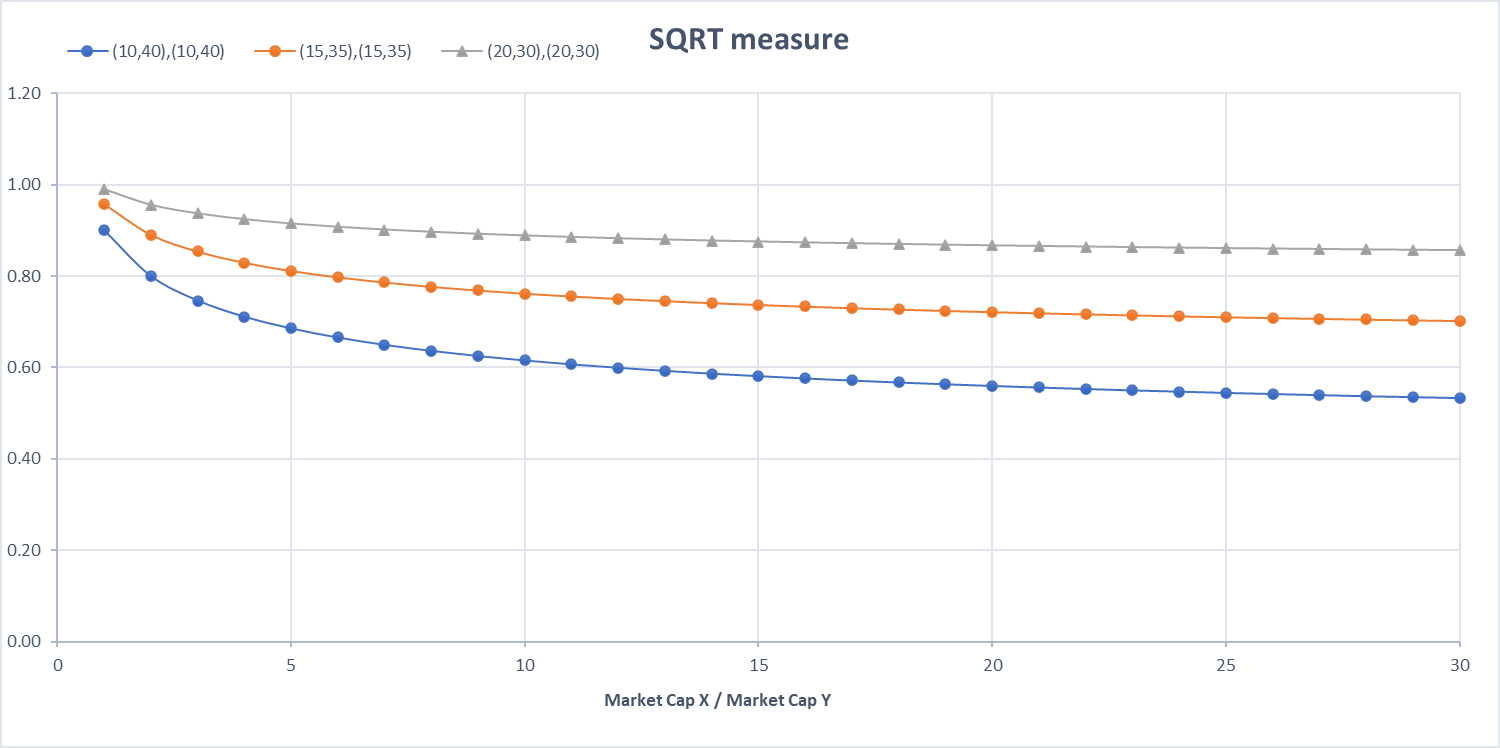
\includegraphics[width=0.85\linewidth]{3.png}
\end{figure}

\begin{figure}[htbp]
\centering
 \caption{ Sum measure for fixed aggregate ownership on different relative market cap ratios}
 \label{sumMarket}
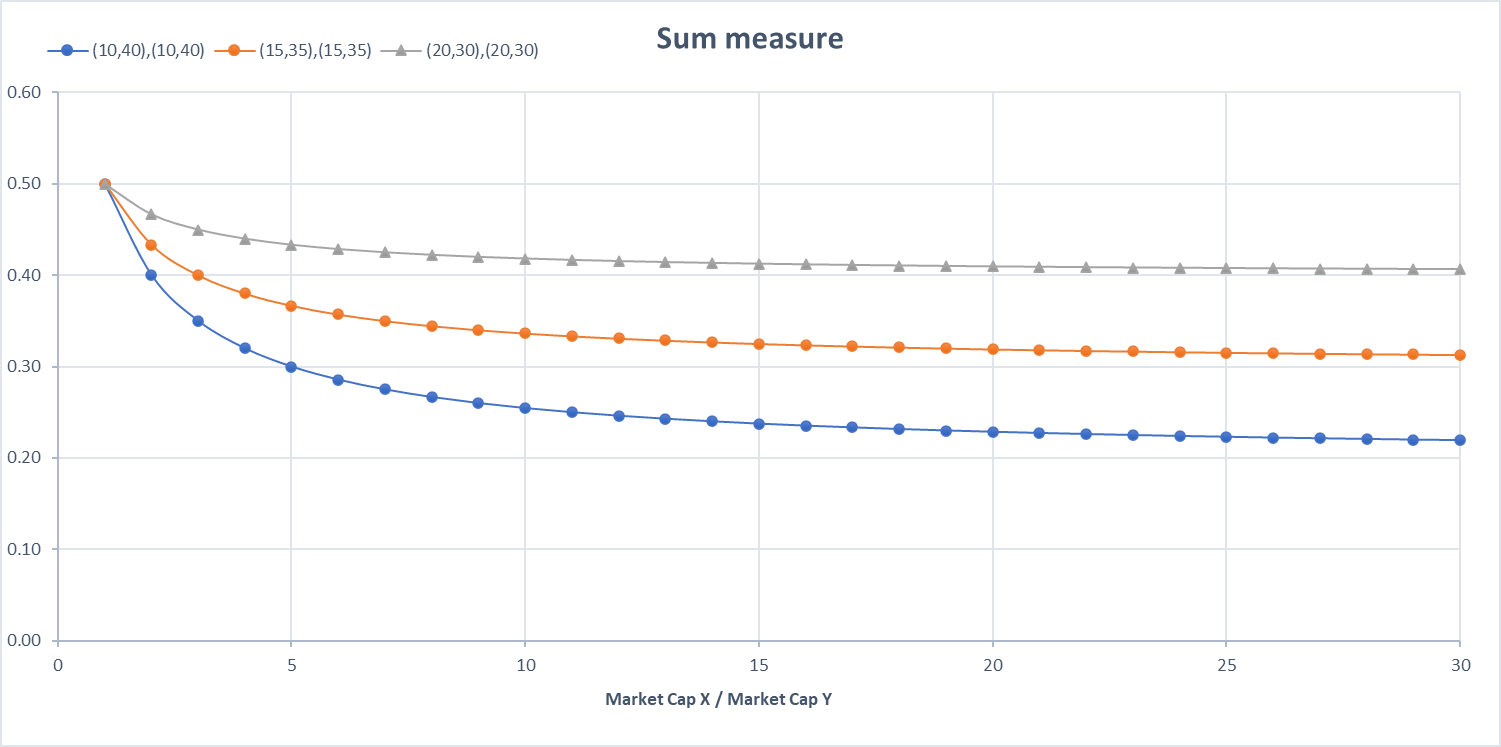
\includegraphics[width=0.85\linewidth]{4.png}
\end{figure}

\begin{table}[htbp]
\centering
\caption{text }
\label{marketcap}
\resizebox{!}{!}
{
          \scriptsize
    \begin{tabular}{ccccccc}
    \hline\hline
  & \multicolumn{6}{c}{\tiny($ \alpha_1 $,$ \beta_1 $),($ \alpha_2 $,$ \beta_2 $) }\\ \cmidrule(lr){2-7}
               & \multicolumn{2}{c}{\tiny(10,40),(10,40)} & \multicolumn{2}{c}{\tiny(15,35),(15,35)} & \multicolumn{2}{c}{\tiny(20,30),(20,30)} \\ \cmidrule(lr){2-3}\cmidrule(lr){4-5}\cmidrule(lr){6-7}
    \tiny $ \frac{\text{MarketCap}_x}{\text{MarketCap}_y} $     &\tiny SQRT  & \tiny SUM   &\tiny SQRT  &\tiny SUM   &\tiny SQRT  &\tiny SUM \\ 
     \hline\addlinespace

         1     & 0.90  & 0.50  & 0.96  & 0.50  & 0.99  & 0.50 \\
         2     & 0.80  & 0.40  & 0.89  & 0.43  & 0.96  & 0.47 \\
         3     & 0.75  & 0.35  & 0.85  & 0.40  & 0.94  & 0.45 \\
         4     & 0.71  & 0.32  & 0.83  & 0.38  & 0.92  & 0.44 \\
         5     & 0.69  & 0.30  & 0.81  & 0.37  & 0.91  & 0.43 \\
         6     & 0.67  & 0.29  & 0.80  & 0.36  & 0.91  & 0.43 \\
         7     & 0.65  & 0.28  & 0.79  & 0.35  & 0.90  & 0.43 \\
         8     & 0.64  & 0.27  & 0.78  & 0.34  & 0.90  & 0.42 \\
         9     & 0.63  & 0.26  & 0.77  & 0.34  & 0.89  & 0.42 \\
         10    & 0.62  & 0.25  & 0.76  & 0.34  & 0.89  & 0.42 \\
     
    \hline\hline
    \end{tabular}
}
\end{table}



In conclusion, We use the SQRT measure for our main study. This measure has an acceptable variation within different distributions and relative market caps. Also, it has a fair value at a lower level of aggregate common ownership. 

On each day, we measure common ownership by SQRT measure and then report an average of these daily calculations for the entire period at the end of each month. We also calculate Anton's measure in this way. Table \ref{measureResults} report snapshots of the distribution of
common ownership measure for both methods. As we expected, the modified measure creates higher values for a high level of common ownership than Anton's measure. The average common ownership measure is five and three times larger, respectively, in business groups and industries.


 \begin{table}[htbp]
      \centering
      \caption{ text}
      \label{measureResults}
      \resizebox{1\textwidth}{!}
      {
      \begin{tabular}{lrrrrrrrrrr}
\toprule
\multirow{2}{*}{Subset}& \multicolumn{5}{c}{MFCAP} & \multicolumn{5}{c}{FCAP} \\
\cmidrule(lr){2-6} \cmidrule(lr){7-11}
&       mean &    std &    min & median &    max &         mean &    std &    min & median &    max \\
\midrule
All               &  0.15 &  0.24 &  0.00 &   0.06 &  4.62 &  0.12 &  0.16 &  0.0 &   0.05 &  0.97 \\
Same Group        &  0.47 &  0.41 &  0.00 &   0.41 &  4.04 &  0.38 &  0.25 &  0.0 &   0.37 &  0.97 \\
Not Same Group    &  0.10 &  0.16 &  0.00 &   0.04 &  2.90 &  0.08 &  0.11 &  0.0 &   0.04 &  0.97 \\
Same Industry     &  0.34 &  0.41 &  0.01 &   0.18 &  4.04 &  0.25 &  0.24 &  0.0 &   0.16 &  0.96 \\
Not Same Industry &  0.12 &  0.19 &  0.00 &   0.05 &  4.62 &  0.10 &  0.14 &  0.0 &   0.05 &  0.97 \\
\bottomrule
\end{tabular}

          }
    \end{table}%





\FloatBarrier





\section{Data and Methodology}



\subsection{Data and Sample}


We gathered industries index and stock returns, trading volume, and other relevant market and accounting data from the Codal website \footnote{\href{http://www.codal.ir}{www.codal.ir}}
 and the  Tehran Securities Exchange Technology Management Co (TSETMC)\footnote{\href{http://www.tsetmc.com}{www.tsetmc.com}} database.
We also use our unique data set, including the daily ownership table that reports all end-of-the-days block-holders of listed firms with their changes in that day.  Block-holder is a shareholder who owns at least 1\% of the total shares outstanding. 

  We exclude ETFs from our listed firms because it has a different return and ownership patterns compared to other firms in our study.
We restrict our empirical analysis to 2015/03-2020/03(1394/01-1398/12 Persian calendar) due to the availability of daily ownership data and the special events \footnote{
The Tehran Stock Exchange's main index (TEPIX) raised exponentially to quadruple value and then fell sharply due to the gigantic entrance of new individual investors that seems to be a bubble period from that period.} that happened after 2020/03, which may affect our results. 
  
  
  
  Business groups - groups of listed firms with interconnected ownership structures controlled by an ultimate common owner - are the principal organizational structure in many parts of the world.
  Business groups seem to be a central feature of corporate ownership in Iran. 
  Most Iranian listed firms present in a complex interlinked shareholders' network that an ultimate owner governs this group through many layers of ownership.{\cite{Aliabadi2022}}  
We do not have pre-specified Iranian business groups despite other countries like South Korea, Japan, and India that their groups are announced formally.
For defining business groups, we use data provided by {\cite{Aliabadi2022}}.
They use \cite{almeida2011structure} algorithm with a 40\% threshold for defining groups. 

\color{red}
Table \ref{t2-1} reports summary statistics of ownership data and business groups. As shown in the table, 494 firms on average have five block-holders that own 73 percent of them. There are 43 business groups on average, with seven members which own 314 (63\%) firms. 
\normalcolor

 \begin{table}[htbp]
        \centering
        \caption{ This table reports summary statistics of ownership features for all the listed firms. At this table by group, we mean business groups.}
        \label{t2-1}
        \resizebox{1\textwidth}{!}
        {
        \begin{tabular}{lrrrrrr}
\toprule
Year &  2014 &  2015 &  2016 &  2017 &  2018 &  2019 \\
\midrule
No. of Firms                        &   365 &   376 &   446 &   552 &   587 &   618 \\
No. of Blockholders                 &  1606 &  1676 &  2099 &  2978 &  3374 &  3416 \\
No. of Groups                       &    38 &    41 &    43 &    44 &    40 &    43 \\
No. of Firms in Groups              &   249 &   268 &   300 &   336 &   346 &   375 \\
Ave. Number of group Members        &     7 &     7 &     7 &     8 &     9 &     9 \\
Ave. ownership of each Blockholders &    18 &    19 &    18 &    17 &    18 &    19 \\
Med. ownership of each Blockholders &     5 &     4 &     4 &     4 &     4 &     4 \\
Ave. Number of Owners               &     7 &     6 &     6 &     7 &     7 &     7 \\
Ave. Block. Ownership               &    77 &    77 &    75 &    76 &    75 &    72 \\
\bottomrule
\end{tabular}

         }
      \end{table}

\subsubsection{Pair composition }
\color{red}
  If two firms have at least one common block-holder, We consider them as a pair. By this definition, there are 9336  unique pairs in entire periods, which is 18\% of possible pairs (597*596/2 = 177906). As we expected, stocks in pairs have concentrated ownership relative to the total sample, and pairs have one common owner.
  
  \normalcolor
  
As one of our empirical studies, we study the impact of being in the same business group relative to being in two distinct groups on pair's correlation.
   For assigning one pair to a group, both firms should belong to one ultimate owner. Another possibility is that each firm belongs to a different ultimate owner or one of them, or both of them do not belong to any groups, which all of them illustrated in figure \ref{g2-1}.
    By classifying pairs, on average, 15\% of them  belong to one business group, and 74\% of them are not in the same business groups  each year. We report summary statistics of ownership features for all pairs in table \ref{t2-2}.
     
 
 \begin{figure}[htbp]
 \centering
\caption{ Three categories for pairs base on being in business groups}
\label{g2-1}

\normalcolor
     \begin{subfigure}[t]{0.9\linewidth}

             \resizebox{0.49\textwidth}{!}{
    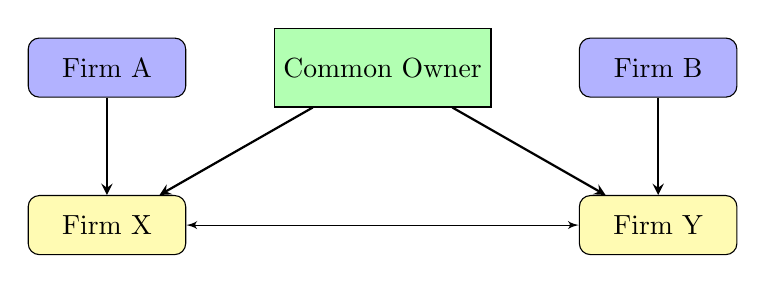
\begin{tikzpicture}[node distance=2cm]
    
    
    
    \node (CH) [process,yshift = -2cm ,xshift=3.5cm] {Common Owner};
    
    \node (end) [startstop1,left of = CH ,xshift=-1.5cm ] {$ \text{Firm A} $};
    
    \node (end2) [startstop1,right of = CH ,yshift=0cm,xshift=1.5cm] {$ \text{Firm B} $};
    
    \node (sur) [startstop2 ,below of = end ,yshift=0cm,xshift=0cm] {$ \text{Firm X} $};
    
    \node (sur2) [startstop2,below of = end2 ,yshift=0cm,xshift=0cm] {$ \text{Firm Y} $};
    
    
    \draw [arrow] (end) --(sur);
    \draw [arrow] (end2) -- (sur2);
    
    
    \draw [arrow] (CH) -- (sur);
    \draw [arrow] (CH) -- (sur2);
    
    \draw [latex'-latex'] (sur) to [bend right =0]  node[sloped, anchor=center, below] {} (sur2);
    
    
    \end{tikzpicture}
     }   
\hfill
\resizebox{0.49\textwidth}{!}{
    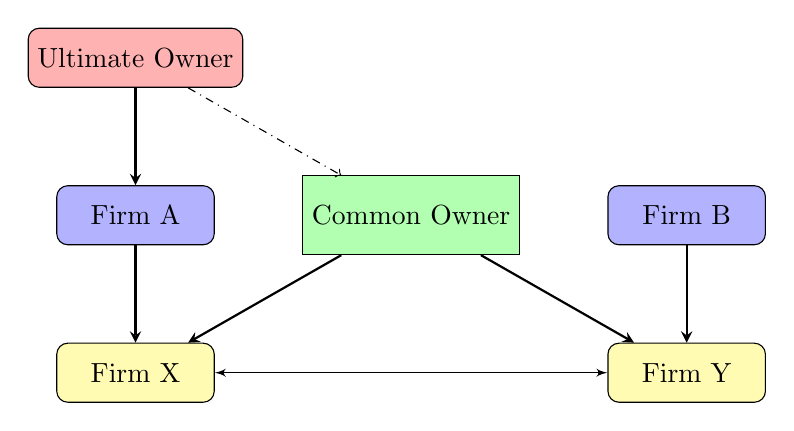
\begin{tikzpicture}[node distance=2cm]
    
    
    \node (start) [startstop] { $ \text{Ultimate Owner} $};
    
    
    \node (CH) [process, below of = start,xshift=3.5cm] {Common Owner};
    
    \node (end) [startstop1,below of = start ] {$ \text{Firm A} $};
    
    \node (end2) [startstop1,right of = CH ,yshift=0cm,xshift=1.5cm] {$ \text{Firm B} $};
    
    \node (sur) [startstop2 ,below of = end ,yshift=0cm,xshift=0cm] {$ \text{Firm X} $};
    
    \node (sur2) [startstop2,below of = end2 ,yshift=0cm,xshift=0cm] {$ \text{Firm Y} $};
    
    
    
    \draw [arrow] (start) --(end);
    
    \draw [arrow] (end) --(sur);
    \draw [arrow] (end2) -- (sur2);
    
    \draw [dash dot,->] (start) -- (CH);
    
    \draw [arrow] (CH) -- (sur);
    \draw [arrow] (CH) -- (sur2);
    
    \draw [latex'-latex'] (sur) to [bend right =0]  node[sloped, anchor=center, below] {} (sur2);
    
    
    \end{tikzpicture}
       }
         \caption{ Pair not in the business group}
       \end{subfigure}
 \bigskip
    \begin{subfigure}[t]{.45\linewidth}
        \centering
        \tiny
            \resizebox{1\textwidth}{!}{
             
        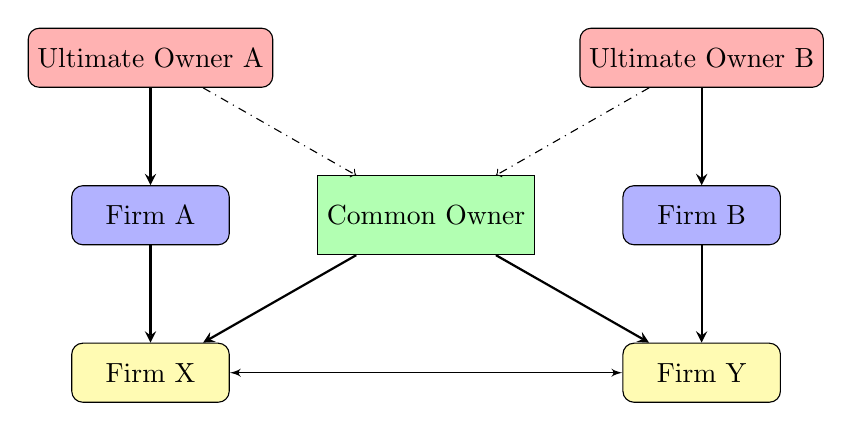
\begin{tikzpicture}[node distance=2cm]
            
            
            \node (start) [startstop] { $ \text{Ultimate Owner A} $};
            \node (start2) [startstop,right of = start,xshift=5cm] {$ \text{Ultimate Owner B} $};
            
            
            \node (CH) [process, below of = start2,xshift=-3.5cm] {Common Owner};
            
            \node (end) [startstop1,below of = start ] {$ \text{Firm A} $};
            
            \node (end2) [startstop1,below of = start2 ,yshift=0cm,xshift=0cm] {$ \text{Firm B} $};
            
            \node (sur) [startstop2 ,below of = end ,yshift=0cm,xshift=0cm] {$ \text{Firm X} $};
            
            \node (sur2) [startstop2,below of = end2 ,yshift=0cm,xshift=0cm] {$ \text{Firm Y} $};
            
            
            
            \draw [arrow] (start) --(end);
            \draw [arrow] (start2) -- (end2);
            
            \draw [arrow] (end) --(sur);
            \draw [arrow] (end2) -- (sur2);
            
            \draw [dash dot,->] (start) -- (CH);
            \draw [dash dot,->] (start2) -- (CH);
            
            \draw [arrow] (CH) -- (sur);
            \draw [arrow] (CH) -- (sur2);
            
            \draw [latex'-latex'] (sur) to [bend right =0]  node[sloped, anchor=center, below] {} (sur2);
            
            
            \end{tikzpicture}
         }   
        \caption{ Pair in two distinct business group}
      \end{subfigure}
      \begin{subfigure}[t]{.45\linewidth}
        \centering
        \tiny
         \resizebox{1\textwidth}{!}{
          
        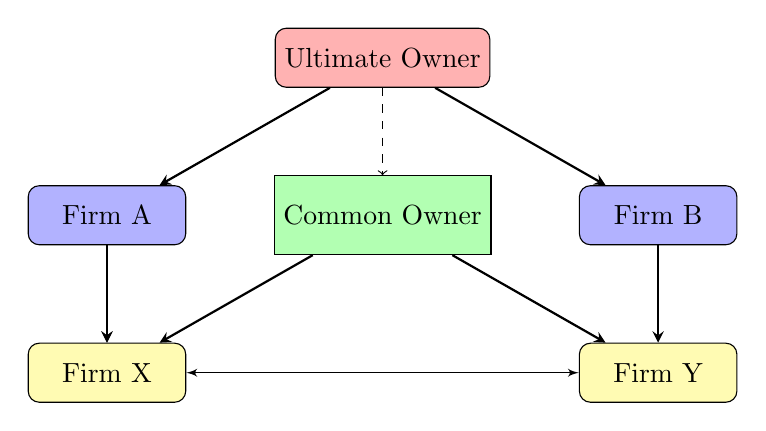
\begin{tikzpicture}[node distance=2cm]
           
           
           \node (start) [startstop] {Ultimate Owner};
           
           
           
           \node (end) [startstop1,below of = start , yshift=0cm , xshift=-3.5cm ] {$ \text{Firm A} $};
           \node (end2) [startstop1,below of = start , yshift=0cm , xshift=3.5cm ] {$ \text{Firm B} $};
           
           
           
           \node (sur) [startstop2 ,below of = end ,yshift=0cm,xshift=0cm] {$ \text{Firm X} $};
           
           
           \node (sur2) [startstop2 ,below of = end2 ,yshift=0cm,xshift=0cm] {$ \text{Firm Y} $};
           
           
           \node (CH) [process, below of = start ,xshift=0] {Common Owner};
           
           
           \draw [arrow] (start) --(end);
           \draw [arrow] (end) --(sur);
           
           \draw [arrow] (start) --(end2);
           
           \draw [arrow] (end) --(sur);
           \draw [arrow] (end2) -- (sur2);
           
           
           \draw [arrow] (CH) -- (sur);
           \draw [arrow] (CH) -- (sur2);
           \draw [dashed ,->] (start) --(CH);
           
           \draw [latex'-latex'] (sur) to [bend right =0]  node[sloped, anchor=center, below] {} (sur2);
           
           
           \end{tikzpicture}
          } 
          
        \caption{ Pair in the same business group}
      \end{subfigure}



   \end{figure}  

  \begin{table}
  \centering
  \caption{ This table reports summary statistics of ownership features for total pairs. At this table by group, we mean business groups.}
  \label{t2-2}
    \resizebox{1\textwidth}{!}
          {
 \begin{tabular}{lrrrrrr}
\toprule
year &   1393 &   1394 &   1395 &   1396 &   1397 &   1398 \\
\midrule
No. of Pairs                          &  20876 &  21187 &  27784 &  41449 &  47234 &  67232 \\
No. of Groups                         &     37 &     40 &     42 &     43 &     39 &     43 \\
No. of Pairs not in Groups            &  11452 &  11192 &  15351 &  26530 &  29182 &  43433 \\
Number of Pairs not in the same Group &   7962 &   8731 &  10971 &  12916 &  15366 &  20745 \\
Number of Pairs in the same Group     &    923 &    955 &   1099 &   1260 &   1536 &   1774 \\
Average Number of Common owner        &      1 &      1 &      1 &      1 &      1 &      1 \\
Med. Number of Common owner           &      1 &      1 &      1 &      1 &      1 &      1 \\
Average Percent of each blockholder   &     19 &     19 &     19 &     19 &     19 &     20 \\
Med. Percent of each blockholder      &     13 &     12 &     12 &     12 &     12 &     14 \\
Average Number of Pairs in one Group  &     31 &     30 &     30 &     34 &     39 &     44 \\
Med. Number of Pairs in one Group     &      8 &     10 &      8 &     10 &      9 &     10 \\
Average Number of Owners              &      5 &      5 &      5 &      5 &      4 &      5 \\
Med. Number of Owners                 &      5 &      5 &      5 &      5 &      4 &      5 \\
Average Block. Ownership              &     73 &     73 &     72 &     70 &     70 &     70 \\
Med. Block. Ownership                 &     73 &     73 &     73 &     71 &     71 &     71 \\
\bottomrule
\end{tabular}

   }
    \end{table}% 

\color{red}
 Figure \ref{g2-2} shows the time series of unique pairs' number in each month. The pattern shows that the portion of pairs that are in one business group is roughly stable. The number of pairs in each period is between 322 to 5101 pairs which, on average, there are 4325 pairs.
 
 \normalcolor
 
\begin{figure}[htbp]
\caption{ The number of unique pairs in each month}
\label{g2-2}
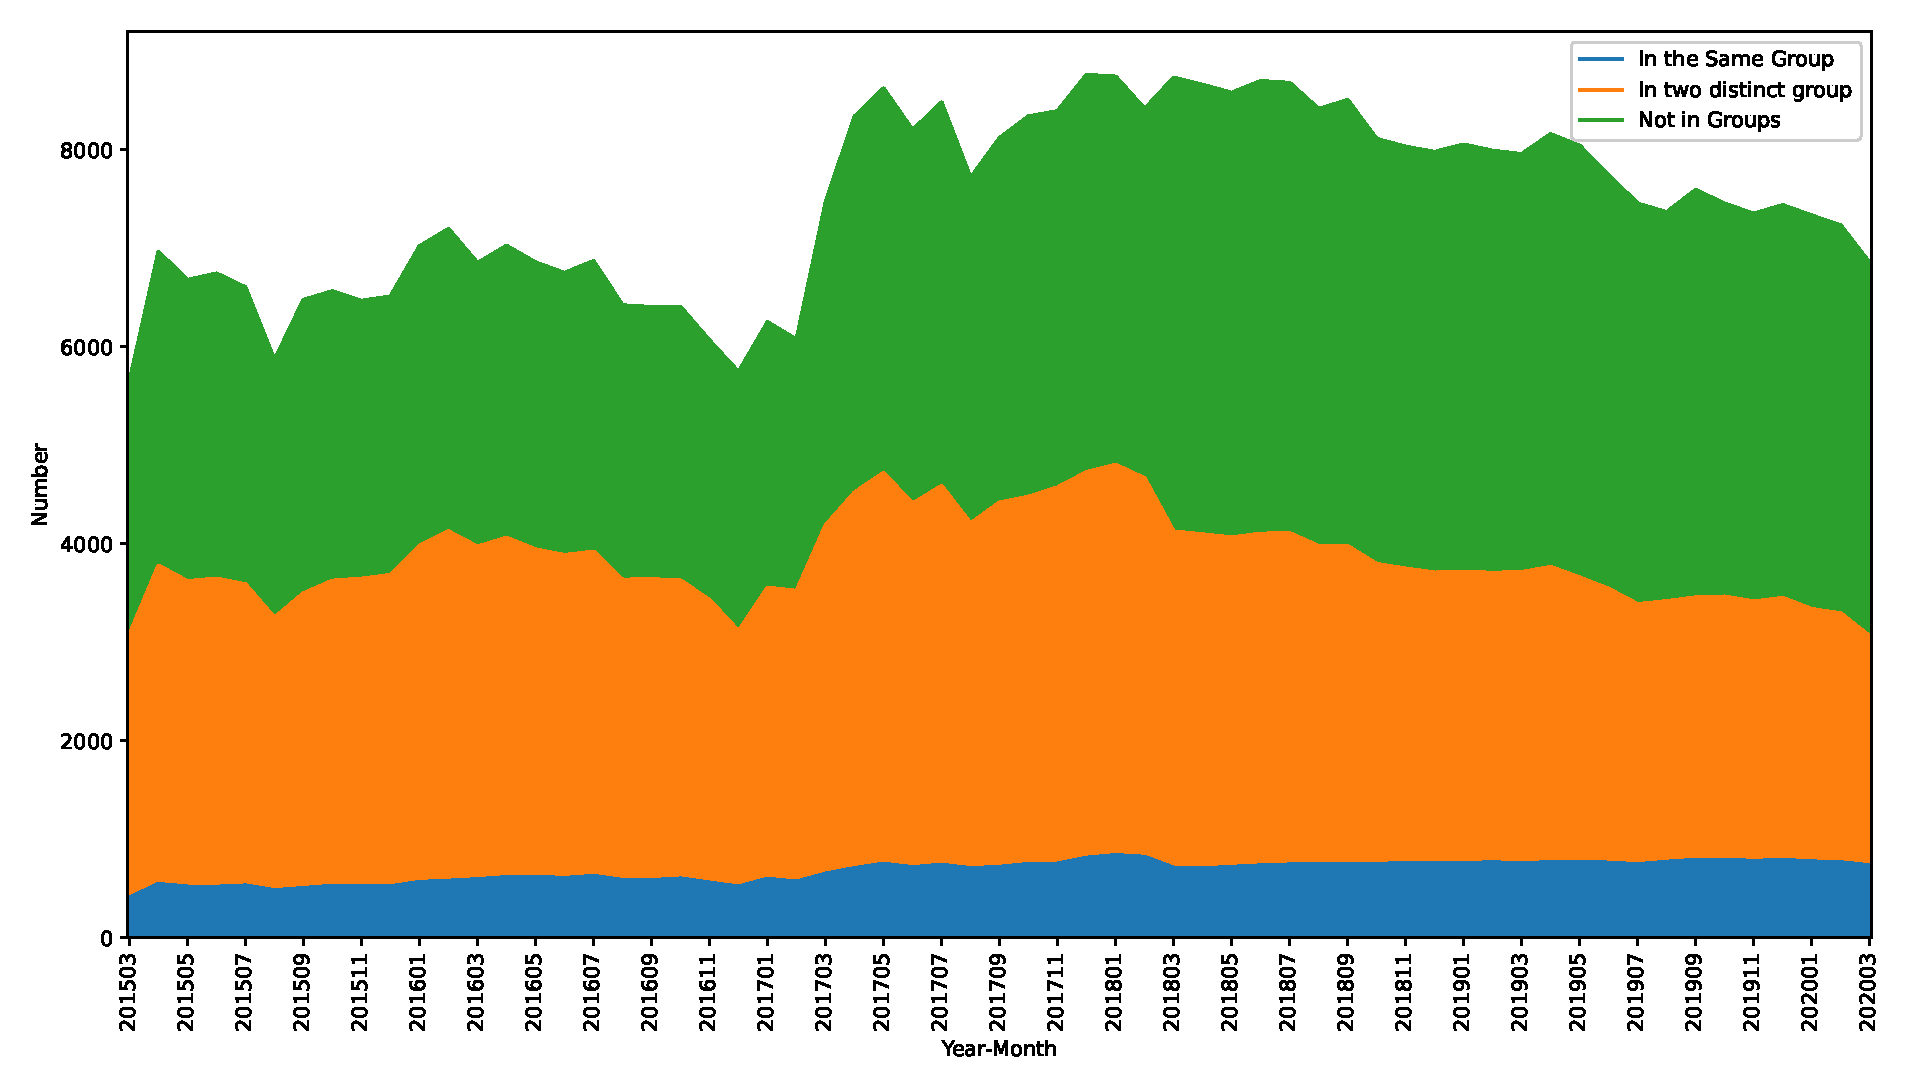
\includegraphics[width=\linewidth]{idMonth.eps}
\end{figure}
 
  \FloatBarrier
  
  
  
\subsubsection{Stock Return comovement}

We calculate the monthly correlation of each pair from stocks' daily abnormal returns. Benchmark for calculating abnormal return is the following equation which is a four-factor model plus industry return due to the importance of industries on stocks' return in the Tehran stock exchange (TSE) :
\begin{equation}
 \begin{split}
   R_{i,t} =\alpha _{i}&+\beta _{mkt,i}{\mathit {R}}_{M,t} + \beta_{Ind,i}{\mathit {R}}_{Ind,t} + \\
  &+\beta _{HML,i}{\mathit {HML}}_{t}+\beta _{SMB,i}{\mathit {SMB}}_{t}+\beta _{UMD,i}{\mathit {UMD}}_{t}+ \varepsilon_{i,t}
  \end{split}
     \label{e5Factor}
\end{equation}
where $ R_{i,t} $, $ R_{M,t} $ and $ R_{Ind,t} $ are excess daily return of respectivly  firm, market and firm's industry from bank deposit's daily rate(risk free). Other variabales difinition is base on Carhart four-factor model [\cite{Carhart4Factor}].

At the end of each month, we estimate our benchmark model base on the past three-month period (from two months before the end of the preceding month) and measure daily residuals.  After that, we calculate the monthly correlation of daily residuals during that month for the pair.

We use other benchmarks for calculating a monthly correlation and report its summary in table \ref{tCorr}. 
As we expected,  models that include industry returns remove pairs' correlation. According to the results, it seems that our selected benchmark (4 Factor + Industry) almost captures all the pairs' comovement because it is nearly a zero mean variable. We use these correlations for our analysis.

     
 \begin{table}[htbp]
        \centering
        \caption{\footnotesize This table reports distribution of calculated correlation base on different models.}
        \label{tCorr}
        \resizebox{1\textwidth}{!}
        {
        \begin{tabular}{lrrrrr}
\toprule
{} &   mean &    std &  min &  median &  max \\
\midrule
 CAPM + Industry    &  0.018 &  0.205 & -1.0 &   0.018 &  1.0 \\
4 Factor            &  0.031 &  0.206 & -1.0 &   0.027 &  1.0 \\
4 Factor + Industry &  0.014 &  0.204 & -1.0 &   0.012 &  1.0 \\
\bottomrule
\end{tabular}

         }
      \end{table}
      

\FloatBarrier
\subsubsection{Controls}
We are interested in the effects of common ownership on pair's comovement.
Our prediction of a higher correlation for a higher level of common ownership dominates by stocks' intrinsic similarity, and these similarities motivate block-holders to hold these stocks simultaneously. These related stocks will comove regardless of who owns them.

The first group of controls is pair controls. These controls include
a dummy variable for whether two stocks are in the same industry, \textbf{SameIndustry}; a dummy variable for whether two stocks are in the same business group, \textbf{SameGroup}. As shown in table \ref{SameGroupIndustry}, 12\% and 11\%  of pairs are in the same industry and business group. 


\begin{table}[htbp]
\caption{\scriptsize This table reports the number of pairs in the same industry and business group.}
\label{SameGroupIndustry}
               \centering \scriptsize
         {

    \begin{tabular}{lcc}\hline\hline
    {Type of Pairs} & {Yes} &{No} \\
    \hline
    \addlinespace
    {SameIndustry} & 1760  & 16739 \\
          & \tiny(10\%) & \tiny (90\%) \\
          \addlinespace
{SameGroup} & 1118  & 17381 \\
          & \tiny(6\%) & \tiny (94\%) \\
          \addlinespace
{SameGroup \& SameIndustry} & 492  & 18007 \\
          & \tiny(3\%) & \tiny (97\%) \\    
                
          \hline\hline
    \end{tabular}%
                 }
             \end{table}


Another group of controls are firm-specific controls.  We define these variables base on  \cite{AntonPolk} methodology. One of these is size control based on the normalized rank-transform of the percentile market capitalization of the two stocks, \textbf{Size1} and \textbf{Size2} (where we label the
larger stock in the pair as the first stock). The other one is a book to market ratio based on the normalized rank-transform of the percentile book to market of the two stocks, \textbf{BookToMarket1} and \textbf{BookToMarket2}.
We also control these characteristics on a pair level. Our measures of similarity, \textbf{SameSize}, and \textbf{SameBookToMarket}, are the negative of the absolute difference in percentile ranking for a particular characteristic across a pair.


We calculate our controls daily and then report the average of these variables for the entire period at the end of each month. Table \ref{ControlsSummary} shows the summary statistics of specified controls in this section.




 \begin{table}[htbp]
 \caption{\scriptsize This table shows the summary statistics of specified controls in empirical studies.}
 \label{ControlsSummary}
               \centering 
               \scriptsize
                \resizebox{\textwidth}{!}  {
    \begin{tabular}{lrrrrrrr}\hline\hline
          & \multicolumn{1}{l}{mean} & \multicolumn{1}{l}{std} & \multicolumn{1}{l}{min} & 25\%  & 50\%  & 75\%  & \multicolumn{1}{l}{max} \\
          \hline
          
          SameIndustry & 0.10  & 0.29  & 0.00  & 0.00  & 0.00  & 0.00  & 1.00 \\
          SameGroup & 0.06  & 0.23  & 0.00  & 0.00  & 0.00  & 0.00  & 1.00 \\
          Size1 & 0.72  & 0.21  & 0.01  & 0.58  & 0.78  & 0.91  & 1.00 \\
          Size2 & 0.43  & 0.25  & 0.00  & 0.23  & 0.42  & 0.62  & 0.99 \\
          SameSize & -0.29 & 0.21  & -0.97 & -0.42 & -0.24 & -0.12 & 0.00 \\
          BookToMarket1 & 0.53  & 0.26  & 0.00  & 0.34  & 0.54  & 0.73  & 1.00 \\
          BookToMarket2 & 0.52  & 0.24  & 0.00  & 0.34  & 0.52  & 0.71  & 1.00 \\
          SameBookToMarket & -0.30 & 0.19  & -0.99 & -0.42 & -0.26 & -0.15 & 0.00 \\
          MonthlyCrossOwnership & 0.01  & 0.05  & 0.00  & 0.00  & 0.00  & 0.00  & 0.96 \\
          
    
    \hline\hline
            \end{tabular}
                 }
             \end{table}
         
         
         
 \begin{figure}[htbp]
 	\caption{}
 	\label{sameIndustryinBG}
 	\centering
 	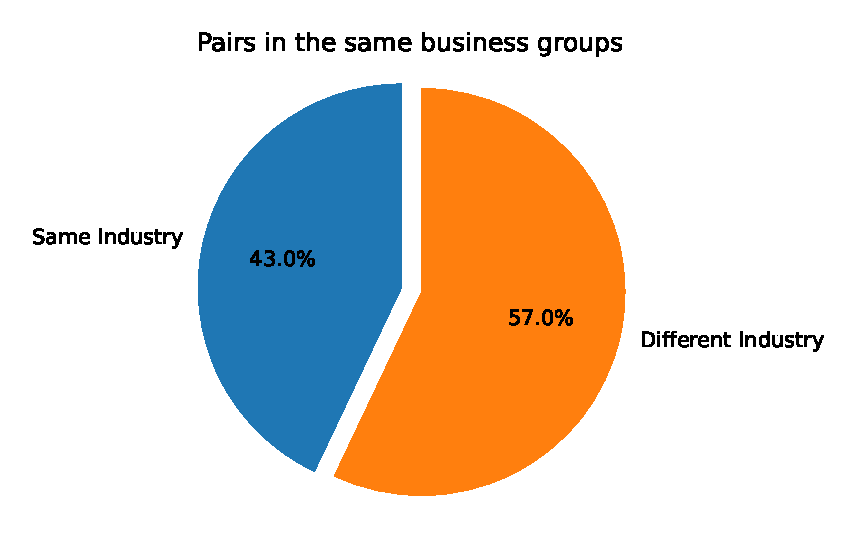
\includegraphics[width=0.48\linewidth]{sameIndustryinBG.eps}
 	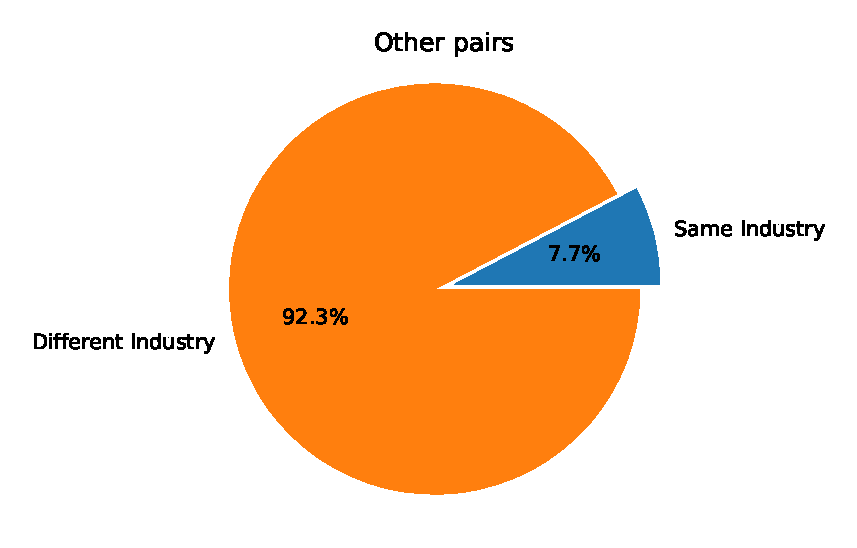
\includegraphics[width=0.48\linewidth]{sameIndustryNoinBG.eps}
 \end{figure}

 \begin{figure}[htbp]
	\caption{}
	\label{BGSummary}
	\centering
	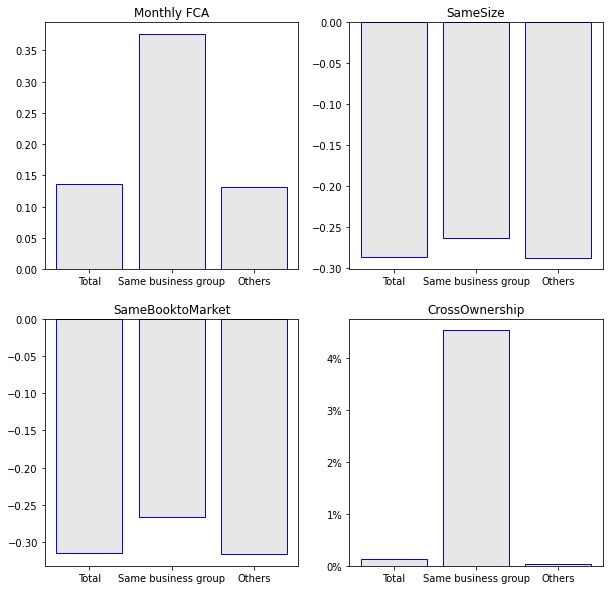
\includegraphics[width=0.85\linewidth]{BGSummary.eps}
\end{figure}



\FloatBarrier
\section{Forecasting Comovement}



 \begin{figure}
 \centering  
\includegraphics[width=0.85\linewidth]{"mcorr50.eps"}
\end{figure}

 \begin{figure}
 \centering  
\includegraphics[width=0.85\linewidth]{"mcorr5l.eps"}
\end{figure}




        


\FloatBarrier
\subsection{Modeling Cross-Sectional Variation in Comovement}


\subsubsection{Model and estimation }

\begin{equation}
\begin{split}
\rho_{ij,t+1} = & \text{ 	}\beta_0 + \beta_1* \text{FCA}^*_{ij,t} + \beta_2* \text{SameGroup}_{ij} \\
 &	+\beta_3* \text{FCA}^*_{ij,t} \times \text{SameGroup}_{ij}   \\
  & + \sum_{k=1} ^{n} \alpha_k*\text{Control}_{ij,t} + \varepsilon_{ij,t+1}
\end{split}
\label{model1}
\end{equation}

\begin{itemize}
\item Use Fama macbeth to estimate 

\item Estimate that model on a monthly frequency 
\item Adjust standard errors by Newey and West adjustment with 4 lags ($ 4(60/100)^{\frac{2}{9}} = 3.57 \sim 4 $)
\item we use current period's correlation as a control variable for controlling omitted variable bias
\end{itemize}

\subsubsection{Results}

\begin{itemize}
\item Use group fixed effect and no change in our results
\item 
\end{itemize}
\FloatBarrier


\begin{table}[htbp]
\centering
\caption{text}
\label{mresult2}
    \resizebox{1\textwidth}{!}{
{
\def\sym#1{\ifmmode^{#1}\else\(^{#1}\)\fi}
\begin{tabular}{l*{7}{c}}
\hline\hline
                &\multicolumn{7}{c}{Dependent Variable: Future Monthly Correlation of 4F+Industry Residuals}                                         \\\cmidrule(lr){2-8}
                &\multicolumn{1}{c}{(1)}         &\multicolumn{1}{c}{(2)}         &\multicolumn{1}{c}{(3)}         &\multicolumn{1}{c}{(4)}         &\multicolumn{1}{c}{(5)}         &\multicolumn{1}{c}{(6)}         &\multicolumn{1}{c}{(7)}         \\
\hline
Same Group      &   0.0138\sym{***}&   0.0128\sym{***}&                  &                  &  0.00978\sym{***}&  0.00458         &  0.00356         \\
                &   (5.76)         &   (6.29)         &                  &                  &   (4.29)         &   (1.43)         &   (1.11)         \\
[1em]
$ \text{FCA*} $ &                  &                  &  0.00405\sym{***}&  0.00375\sym{***}&  0.00296\sym{***}&  0.00258\sym{***}&  0.00273\sym{***}\\
                &                  &                  &   (4.94)         &   (5.12)         &   (3.77)         &   (3.53)         &   (3.51)         \\
[1em]
 $ (\text{FCA}^*) \times {\text{SameGroup} }  $ &                  &                  &                  &                  &                  &  0.00524\sym{**} &  0.00517\sym{**} \\
                &                  &                  &                  &                  &                  &   (3.21)         &   (3.18)         \\
\hline
Observations    &   388492         &   388492         &   388492         &   388492         &   388492         &   388492         &   388492         \\
Group Effect    &       No         &       No         &       No         &       No         &       No         &       No         &      Yes         \\
Controls        &       No         &      Yes         &       No         &      Yes         &      Yes         &      Yes         &      Yes         \\
$ R^2 $         & 0.000404         &  0.00200         & 0.000423         &  0.00201         &  0.00229         &  0.00245         &  0.00875         \\
\hline\hline
\multicolumn{8}{l}{\footnotesize \textit{t} statistics in parentheses}\\
\multicolumn{8}{l}{\footnotesize \sym{*} \(p<0.05\), \sym{**} \(p<0.01\), \sym{***} \(p<0.001\)}\\
\end{tabular}
}

}
\end{table}


\FloatBarrier
%\subsubsection{Bearish/Bullish Market }
%
%
%\begin{equation}
\begin{split}
\rho_{ij,t+1} = & \text{ 	}\beta_0 + \beta_1*\text{FCA}^*_{ij,t}\\
& +\beta_2 * {\text{Bearish Market} } \times {\text{SameGroup} }  \\
& + 
\beta_3 *{\text{Bullish Market} } \times {\text{SameGroup} }\\
& 
 + \beta_4 * \text{FCA}^*_{ij,t} \times {\text{Bearish Market} } \times {\text{SameGroup} }\\
&
+ \beta_5 * \text{FCA}^*_{ij,t} \times {\text{Bullish Market} } \times {\text{SameGroup} }\\
  & + \sum_{k=1} ^{n} \alpha_k*\text{Control}_{ij,t} + \varepsilon_{ij,t+1}
\end{split}
\end{equation}
%
%
%
%\begin{itemize}
%\item Use Fama macbeth to estimate 
%
%\item Estimate that model on a monthly frequency 
%\item Adjust standard errors by Newey and West adjustment with 4 lags ($ 4(60/100)^{\frac{2}{9}} = 3.57 \sim 4 $)
%\item we use current period's correlation as a control variable for controlling omitted variable bias
%\end{itemize}
%
%\subsubsection{Results}
%
%\begin{itemize}
%\item 37\% of observations are in bearish market
%\item In table \ref{mresult2Down} we use a time dummy for a bearish market and a bullish market in the next period. We also interact with these dummies with our interested controls. According to results, in a bearish market, only high common ownerships in the business group affect the pair's correlation. However, in a bullish market, all level of common ownership that happens in the same business group has a great effect on the pair's correlation
%\end{itemize}
%
%
%
%
%\begin{table}[htbp]
%\centering
%\caption{text}
%\label{mresult2Down}
%    \resizebox{1\textwidth}{!}{
%{
\def\sym#1{\ifmmode^{#1}\else\(^{#1}\)\fi}
\begin{tabular}{l*{3}{c}}
\hline\hline
                &\multicolumn{3}{c}{Fu. Monthly Cor. of 4F+Ind. Residuals}\\\cmidrule(lr){2-4}
                &\multicolumn{1}{c}{(1)}         &\multicolumn{1}{c}{(2)}         &\multicolumn{1}{c}{(3)}         \\
\hline
$ \text{FCA*} $ & 0.000548         & 0.000548         & 0.000704         \\
                &   (0.80)         &   (0.80)         &   (1.04)         \\
[1em]
 $ (\text{FCA}^*) \times {\text{SameGroup} }  $ &  0.00744\sym{**} &  0.00744\sym{**} &                  \\
                &   (3.32)         &   (3.32)         &                  \\
[1em]
SameGroup       &  0.00952\sym{**} &  0.00266         &  0.00495\sym{*}  \\
                &   (2.73)         &   (1.45)         &   (2.14)         \\
[1em]
$ {\text{Bearish Market} } \times {\text{SameGroup} }  $ &                  & 0.000595         & 0.000595         \\
                &                  &   (0.53)         &   (0.53)         \\
[1em]
$ {\text{Bullish Market} } \times {\text{SameGroup} }  $ &                  &  0.00626\sym{**} &  0.00626\sym{**} \\
                &                  &   (2.81)         &   (2.81)         \\
[1em]
$ (\text{FCA}^*) \times {\text{Bullish Market}} \times {\text{SameGroup} }  $ &                  &                  &  0.00294         \\
                &                  &                  &   (1.99)         \\
[1em]
$ (\text{FCA}^*) \times {\text{Bearish Market}} \times {\text{SameGroup} }  $ &                  &                  &  0.00228\sym{*}  \\
                &                  &                  &   (2.51)         \\
\hline
Observations    &   434850         &   434850         &   434850         \\
\(R^{2}\)       &    0.037         &    0.037         &    0.037         \\
\hline\hline
\multicolumn{4}{l}{\footnotesize \textit{t} statistics in parentheses}\\
\multicolumn{4}{l}{\footnotesize \sym{*} \(p<0.05\), \sym{**} \(p<0.01\), \sym{***} \(p<0.001\)}\\
\end{tabular}
}

%}
%\end{table}
%
%
%\FloatBarrier
\subsection{Discontinuity}

 \begin{figure}[htbp]
 \centering  
\includegraphics[width=0.85\linewidth]{"Qmcorr5lrd.eps"}
\end{figure}

 \begin{figure}[htbp]
	\centering  
	\includegraphics[width=0.85\linewidth]{"Qmcorr5subsample.eps"}
\end{figure}

 \begin{figure}[htbp]
	\centering  
	\includegraphics[width=0.85\linewidth]{"Qmcorr5lrdbgsubsample.eps"}
\end{figure}


 \begin{figure}[htbp]
	\centering  
	\includegraphics[width=\linewidth]{"QarterSummary.eps"}
\end{figure}

	\begin{figure}   
	\centering
	\includegraphics[width=0.45\linewidth]{"sameIndustryinQuarter.eps"}
	\includegraphics[width=0.45\linewidth]{"sameIBGinQuarter.eps"}
\end{figure}
\FloatBarrier

\subsubsection{Model and estimation}

\begin{equation}
\begin{split}
\rho_{ij,t+1} = & \text{ 	}\beta_0 + \beta_1* (\text{FCA}^*_{ij,t} > Q3[\text{FCA}^*_{ij,t}])  + \beta_2 * \text{SameGroup}_{ij}  \\
& +  \beta_3* (\text{FCA}^*_{ij,t} > Q3[\text{FCA}^*_{ij,t}]) \times \text{SameGroup}_{ij}   \\
  & + \sum_{k=1} ^{n} \alpha_k*\text{Control}_{ij,t} + \varepsilon_{ij,t+1}
\end{split}
\label{model2}
\end{equation}

\begin{itemize}
\item refer to table \ref{ControlsCorr} high correlation between $ (\text{FCA}^* > Q3[\text{FCA}^*]) \times  (\text{FCA}^*) \times {\text{SameGroup}} $ and $ (\text{FCA}^*) \times {\text{SameGroup}} $
\end{itemize}

%\begin{table}[htbp]
%\centering
%\caption{text}
%\label{ControlsCorr}
%\resizebox{1\textwidth}{!}{
%
\begin{tabular}{lccccccccccc}
\hline\hline
Correlation      & \multicolumn{1}{l}{(1)} & \multicolumn{1}{l}{(2)} & \multicolumn{1}{l}{(3)} & \multicolumn{1}{l}{(4)} & \multicolumn{1}{l}{(5)} & \multicolumn{1}{l}{(6)} & \multicolumn{1}{l}{(7)} & \multicolumn{1}{l}{(8)} & \multicolumn{1}{l}{(9)} & \multicolumn{1}{l}{(10)} & \multicolumn{1}{l}{(11)} \\
\hline\addlinespace
    (1) $\rho_f$ & 1.00  &       &       &       &       &       &       &       &       &       & \\\addlinespace
    (2) $\rho$ & 0.11  & 1.00  &       &       &       &       &       &       &       &       & \\\addlinespace
    (3) $ \text{FCA*} $ & 0.02  & 0.01  & 1.00  &       &       &       &       &       &       &       & \\\addlinespace
    (4) $ (\text{FCA}^* > Q3[\text{FCA}^*]) $ & 0.02  & 0.02  & \boxed{0.75}  & 1.00  &       &       &       &       &       &       & \\\addlinespace
    (5) $ (\text{FCA}^* > Q3[\text{FCA}^*]) \times {\text{FCA} ^*}  $  & 0.02  & 0.02  & \boxed{0.76}  & \boxed{0.98}  & 1.00  &       &       &       &       &       & \\\addlinespace
     (6) $ (\text{FCA}^*) \times {\text{SameGroup} }  $ & 0.03  & 0.03  & 0.55  & 0.60  & 0.68  & 1.00  &       &       &       &       & \\\addlinespace
    (7) $ (\text{FCA}^* > Q3[\text{FCA}^*]) \times  (\text{FCA}^*) \times {\text{SameGroup}} $ & 0.03  & 0.03  & 0.53  & 0.63  & \boxed{0.71}  & \boxed{0.95}  & 1.00  &       &       &       & \\\addlinespace
    (8) SameGroup & 0.03  & 0.03  & 0.44  & 0.49  & 0.54  & \boxed{0.75}  & \boxed{0.82}  & 1.00  &       &       & \\\addlinespace
    (9) SameIndustry & 0.01  & 0.01  & 0.28  & 0.30  & 0.32  & 0.33  & 0.36  & 0.38  & 1.00  &       & \\\addlinespace
    (10) SameSize & 0.01  & 0.01  & 0.12  & 0.12  & 0.12  & 0.06  & 0.07  & 0.03  & 0.12  & 1.00  & \\\addlinespace
    (11) SameBookToMarket & 0.01  & 0.01  & 0.02  & 0.03  & 0.04  & 0.05  & 0.06  & 0.06  & 0.11  & 0.07  & 1.00\\\addlinespace
    
\hline\hline
\end{tabular}%
%}
%\end{table}

\subsubsection{Results}
\begin{table}[htbp]
\centering
\caption{\scriptsize}
\label{Qmresult2}
    \resizebox{0.8\textwidth}{!}{
{
\def\sym#1{\ifmmode^{#1}\else\(^{#1}\)\fi}
\begin{tabular}{l*{6}{c}}
\hline\hline
                &\multicolumn{6}{c}{Dep. Variable: Future Monthly Corr. of 4F+Ind. Residuals}                                     \\\cmidrule(lr){2-7}
                &\multicolumn{1}{c}{(1)}         &\multicolumn{1}{c}{(2)}         &\multicolumn{1}{c}{(3)}         &\multicolumn{1}{c}{(4)}         &\multicolumn{1}{c}{(5)}         &\multicolumn{1}{c}{(6)}         \\
\hline
$ \text{FCA*} $ &  0.00405\sym{***}& 0.000173         & 0.000194         & 0.000177         & 0.000105         &-0.00000621         \\
                &   (4.94)         &   (0.17)         &   (0.20)         &   (0.18)         &   (0.11)         &  (-0.01)         \\
[1em]
 $ (\text{FCA} > Q3[\text{FCA}]) \times {\text{FCA} ^*}  $ &                  &  0.00875\sym{***}&  0.00846\sym{***}&  0.00683\sym{***}&  0.00724\sym{***}&  0.00799\sym{***}\\
                &                  &   (4.36)         &   (4.36)         &   (3.65)         &   (3.91)         &   (4.42)         \\
[1em]
Same Group      &                  &                  &                  &  0.00730\sym{**} &  0.00707\sym{**} &  0.00552\sym{*}  \\
                &                  &                  &                  &   (3.21)         &   (3.19)         &   (2.40)         \\
[1em]
 $ {\rho\_t} $   &                  &                  &   0.0239\sym{***}&   0.0238\sym{***}&   0.0238\sym{***}&   0.0234\sym{***}\\
                &                  &                  &   (6.95)         &   (6.96)         &   (6.98)         &   (7.03)         \\
[1em]
SameIndustry    &                  &                  &                  &                  & -0.00467\sym{**} & -0.00493\sym{**} \\
                &                  &                  &                  &                  &  (-2.90)         &  (-3.06)         \\
[1em]
SameSize        &                  &                  &                  &                  &  0.00830\sym{***}&  0.00904\sym{***}\\
                &                  &                  &                  &                  &   (4.06)         &   (4.05)         \\
[1em]
SameBookToMarket&                  &                  &                  &                  &  0.00481\sym{*}  &  0.00517\sym{*}  \\
                &                  &                  &                  &                  &   (2.44)         &   (2.36)         \\
[1em]
CrossOwnership  &                  &                  &                  &                  &   0.0254\sym{*}  &   0.0238         \\
                &                  &                  &                  &                  &   (2.12)         &   (1.84)         \\
\hline
Observations    &   388492         &   388492         &   388492         &   388492         &   388492         &   388492         \\
Group FE        &       No         &       No         &       No         &       No         &       No         &      Yes         \\
$ R^2 $         & 0.000423         & 0.000765         &  0.00163         &  0.00185         &  0.00256         &  0.00885         \\
\hline\hline
\multicolumn{7}{l}{\footnotesize \textit{t} statistics in parentheses}\\
\multicolumn{7}{l}{\footnotesize \sym{*} \(p<0.05\), \sym{**} \(p<0.01\), \sym{***} \(p<0.001\)}\\
\end{tabular}
}

}
\end{table}
%\begin{table}[htbp]
%\centering
%\caption{\scriptsize}
%\label{Qmresult3}
%    \resizebox{0.8\textwidth}{!}{
%{
\def\sym#1{\ifmmode^{#1}\else\(^{#1}\)\fi}
\begin{tabular}{l*{7}{c}}
\hline\hline
                &\multicolumn{7}{c}{Dep. Variable: Future Monthly Correlation of 4F+Industry Residuals}                                              \\\cmidrule(lr){2-8}
                &\multicolumn{1}{c}{(1)}         &\multicolumn{1}{c}{(2)}         &\multicolumn{1}{c}{(3)}         &\multicolumn{1}{c}{(4)}         &\multicolumn{1}{c}{(5)}         &\multicolumn{1}{c}{(6)}         &\multicolumn{1}{c}{(7)}         \\
\hline
$ \text{FCA*} $ & 0.000105         &  0.00258\sym{***}&  0.00251\sym{**} &0.0000530         &  0.00259\sym{***}& 0.000151         & 0.000209         \\
                &   (0.11)         &   (3.53)         &   (3.24)         &   (0.06)         &   (3.57)         &   (0.15)         &   (0.24)         \\
[1em]
 $ (\text{FCA} > Q3[\text{FCA}]) \times {\text{FCA} ^*}  $ &  0.00724\sym{***}&                  &                  &  0.00677\sym{**} &                  &  0.00641\sym{**} &  0.00634\sym{**} \\
                &   (3.91)         &                  &                  &   (3.45)         &                  &   (3.23)         &   (3.24)         \\
[1em]
 $ (\text{FCA}^*) \times {\text{SameGroup} }  $ &                  &  0.00524\sym{**} &                  &  0.00322         & -0.00506         &                  & -0.00272         \\
                &                  &   (3.21)         &                  &   (1.76)         &  (-0.95)         &                  &  (-0.52)         \\
[1em]
 $ (\text{FCA} > Q3[\text{FCA}]) \times  (\text{FCA}^*) \times {\text{SameGroup}&                  &                  &  0.00931\sym{***}&                  &   0.0155\sym{*}  &  0.00579\sym{*}  &  0.00927         \\
                &                  &                  &   (3.83)         &                  &   (2.09)         &   (2.17)         &   (1.27)         \\
\hline
Observations    &   388492         &   388492         &   388492         &   388492         &   388492         &   388492         &   388492         \\
\(R^{2}\)       &    0.003         &    0.002         &    0.002         &    0.003         &    0.003         &    0.003         &    0.003         \\
\hline\hline
\multicolumn{8}{l}{\footnotesize \textit{t} statistics in parentheses}\\
\multicolumn{8}{l}{\footnotesize \sym{*} \(p<0.05\), \sym{**} \(p<0.01\), \sym{***} \(p<0.001\)}\\
\end{tabular}
}

%}
%\end{table}

\begin{table}[htbp]
	\centering
	\caption{\scriptsize}
	\label{Qmresult2subsanple}
	\resizebox{0.8\textwidth}{!}{
		{
\def\sym#1{\ifmmode^{#1}\else\(^{#1}\)\fi}
\begin{tabular}{l*{6}{c}}
\hline\hline
                &\multicolumn{6}{c}{Dependent Variable: Future Monthly Correlation of 4F+Industry Residuals}                      \\\cmidrule(lr){2-7}
                &\multicolumn{1}{c}{(1)}         &\multicolumn{1}{c}{(2)}         &\multicolumn{1}{c}{(3)}         &\multicolumn{1}{c}{(4)}         &\multicolumn{1}{c}{(5)}         &\multicolumn{1}{c}{(6)}         \\
\hline
$ \text{FCA*} $ &   0.0302\sym{***}&   0.0283\sym{***}&   0.0241\sym{***}&   0.0215\sym{***}&   0.0208\sym{***}&   0.0156\sym{**} \\
                &   (5.38)         &   (5.27)         &   (4.59)         &   (3.74)         &   (3.68)         &   (2.76)         \\
[1em]
Same Group      &                  &                  &                  &  0.00382         &  0.00337         &  0.00285         \\
                &                  &                  &                  &   (1.52)         &   (1.32)         &   (0.95)         \\
[1em]
 $ {\rho_t} $   &                  &   0.0545\sym{***}&   0.0544\sym{***}&   0.0544\sym{***}&   0.0539\sym{***}&   0.0533\sym{***}\\
                &                  &   (9.47)         &   (9.49)         &   (9.49)         &   (9.51)         &   (9.69)         \\
[1em]
SameIndustry    &                  &                  &  0.00862\sym{***}&  0.00806\sym{**} &  0.00564\sym{**} &  0.00699\sym{**} \\
                &                  &                  &   (3.56)         &   (3.27)         &   (2.72)         &   (2.92)         \\
[1em]
SameSize        &                  &                  &                  &                  &  0.00609         &  0.00773         \\
                &                  &                  &                  &                  &   (1.10)         &   (1.45)         \\
[1em]
SameBookToMarket&                  &                  &                  &                  &   0.0213\sym{***}&   0.0208\sym{***}\\
                &                  &                  &                  &                  &   (4.60)         &   (4.35)         \\
[1em]
CrossOwnership  &                  &                  &                  &                  &   0.0335         &   0.0239         \\
                &                  &                  &                  &                  &   (1.83)         &   (1.29)         \\
\hline
Observations    &    97528         &    97528         &    97528         &    97528         &    97528         &    97528         \\
Group FE        &       No         &       No         &       No         &       No         &       No         &      Yes         \\
$ R^2 $         &  0.00143         &  0.00552         &  0.00645         &  0.00722         &  0.00954         &   0.0324         \\
\hline\hline
\multicolumn{7}{l}{\footnotesize \textit{t} statistics in parentheses}\\
\multicolumn{7}{l}{\footnotesize \sym{*} \(p<0.05\), \sym{**} \(p<0.01\), \sym{***} \(p<0.001\)}\\
\end{tabular}
}

	}
\end{table}



%\begin{landscape}
%
%\begin{table}[p]
%\caption{\scriptsize}
%\label{Qmresult4}
%    \resizebox{1.5\textwidth}{!}{
%{
\def\sym#1{\ifmmode^{#1}\else\(^{#1}\)\fi}
\begin{tabular}{l*{8}{c}}
\hline\hline
                &\multicolumn{8}{c}{Dependent Variable: Future Monthly Correlation of 4F+Ind. Res.}                                                                     \\\cmidrule(lr){2-9}
                &\multicolumn{1}{c}{(1)}         &\multicolumn{1}{c}{(2)}         &\multicolumn{1}{c}{(3)}         &\multicolumn{1}{c}{(4)}         &\multicolumn{1}{c}{(5)}         &\multicolumn{1}{c}{(6)}         &\multicolumn{1}{c}{(7)}         &\multicolumn{1}{c}{(8)}         \\
\hline
$ \text{FCA*} $ & 0.000377         & 0.000698         &-0.000175         &  0.00199\sym{***}&  0.00177\sym{**} & -0.00151         & -0.00177         &-0.0000771         \\
                &   (0.65)         &   (1.25)         &  (-0.31)         &   (3.56)         &   (3.00)         &  (-1.58)         &  (-1.84)         &  (-0.14)         \\
[1em]
Same Group      &  0.00624\sym{**} &   0.0102\sym{***}& -0.00153         &   0.0117\sym{***}&  0.00661\sym{*}  &   0.0366\sym{***}&   0.0268\sym{***}&  0.00750\sym{***}\\
                &   (2.81)         &   (3.95)         &  (-0.53)         &   (3.76)         &   (2.15)         &  (10.31)         &   (6.57)         &   (3.53)         \\
[1em]
 $ (\text{FCA}^*) \times {\text{SameGroup} }  $ &  0.00992\sym{***}&                  &   0.0134\sym{***}&                  &  0.00599\sym{*}  &                  &   0.0123\sym{***}&   0.0105\sym{***}\\
                &   (6.49)         &                  &   (4.80)         &                  &   (2.34)         &                  &   (4.17)         &   (6.72)         \\
\hline
Observations    &  1665996         &   346170         &   346170         &   693728         &   693728         &   626098         &   626098         &  1665996         \\
Controls        &      Yes         &      Yes         &      Yes         &      Yes         &      Yes         &      Yes         &      Yes         &      Yes         \\
Sub-sample      &All Firms         &Big Firms         &Big Firms         &Big \& Small Firms         &Big \& Small Firms         &Small Firms         &Small Firms         &All Firms         \\
Pair Size FE    &       No         &       No         &       No         &       No         &       No         &       No         &       No         &      Yes         \\
$ R^2 $         & 0.000898         &  0.00193         &  0.00232         &  0.00135         &  0.00149         &  0.00180         &  0.00198         &  0.00130         \\
\hline\hline
\multicolumn{9}{l}{\footnotesize \textit{t} statistics in parentheses}\\
\multicolumn{9}{l}{\footnotesize \sym{*} \(p<0.05\), \sym{**} \(p<0.01\), \sym{***} \(p<0.001\)}\\
\end{tabular}
}

%}
%\end{table}
%\end{landscape}

\FloatBarrier
\section{Forecasting Comovement the Presence of Business Groups}
\FloatBarrier
\subsection{Overview of Business Groups in Tehran Stock Exchange}

There is no difference between emerging markets (such as  Chile, India, Indonesia, South Korea, Pakistan, and many more) and developed ones (like Italy and Sweden); business groups present everywhere. However, group-affiliated firms are relatively large and economically important in emerging markets. 
These groups principally consist of legally independent firms grouped by persistent formal (e.g., equity) and informal (e.g., family) links.(\cite{Khanna2007}) 
There is a complex ownership network in TSE as an emerging market. 
This complicated ownership creates a vast number of business groups in which an ultimate owner controls them through a multi-layer of ownership. (\cite{FirmInterlock})




The reason for many of these business groups back to the 1979 revolution. After the revolution, due to social sentiment, critical sectors of the economy nationalized, and their ownership transferred to the government or other pseudo-government foundations. Also,
some other groups of firms in heavy industries were established and controlled by the Industrial Development and Renovation Organization (IDRO) during the 1960s and 1970s.  (IDRO was a state-owned holding company for investing in capital-intensive industries) 

The business groups are formed from mentioned ancestors due to two related forces; A multi-phased privatization by the state and the development of the domestic stock market. In the first wave of privatization, more than 300 companies were fully or partially privatized. In the second one, approximately  \$150 billion ownership of State-Owned Enterprises (SOEs) and assets were transferred.  
Pension funds, military institutions, cultural and religious foundations, and revolutionary foundations (pseudo-government groups) primary customers in the second wave of privatization. These waves of privatization transferred control of hundreds of SOEs to
semi-governmental groups and were the main driver of the formation of business groups in Iran. In addition, the developing stock market from the early 2000s enhances this effect. The government tried to develop the stock market as a tool for better privatization. 
(\cite{Aliabadi2022})

In conclusion, the multiple waves of privatization with the development of the stock market changed ownership structure in pre-revolutionary holding companies and post-revolutionary foundations and creat large business groups that govern primary  industries.































\FloatBarrier
\subsection{Modeling Cross-Sectional Variation in Comovement in Business Groups}
  \begin{figure}   
 \centering
\includegraphics[width=0.85\linewidth]{"mcorr5bg.eps"}     \end{figure}    

 \begin{figure}
 \centering  
\includegraphics[width=0.85\linewidth]{"Qmcorr5lrdbg.eps"}
\end{figure}
%
%\subsubsection{Effective Business Group}
% \begin{equation*}
 \scriptsize
 \begin{split}
 \rho_{ij,t+1} = & \text{ 	}\beta_0   + \beta_1* \text{FCA}_{ij,t}^*  + \beta_2 * \text{SameGroup}_{ij} + \sum_1^G \lambda_{1,g} *\gamma_{g}\\
 &   + \sum_1^G \lambda_{2,g} * \text{SameGroup}_{ij} * \gamma_g + \sum_1^G \lambda_{3,g} *  \gamma_g  * \text{FCA}_{ij,t}^*  \\
  & + \sum_1^G \lambda_{4,g} \text{SameGroup}_{ij} * \gamma_g  * \text{FCA}_{ij,t}^*  + \sum_{k=1} ^{n} \alpha_k*\text{Control}_{ij,t} + \varepsilon_{ij,t+1}
 \end{split}
 \end{equation*}
%
%
%
%
%
%\subsubsection{Check presence of Banks in Groups}
%
%\begin{equation*}
\scriptsize
\begin{split}
\rho_{ij,t+1} = & \text{ 	}\beta_0   + \beta_1* \text{FCA}_{ij,t}^*  + \beta_2 * \text{SameGroup}_{ij} 	\\
 &+\beta_3 * \text{FCA}_{ij,t}^* *\ \text{SameGroup}_{ij}  + \beta_{10} *\text{Bank In Group} + \beta_{11}*\text{Bank in group} \\
  & + \beta_4 * \text{Bank In Group}*\ \text{SameGroup}_{ij}  + \beta_5 * \text{Bank In Group}* \text{SameGroup}_{ij} * \text{FCA}_{ij,t}^*  \\
   &+ \sum_{k=1} ^{n} \alpha_k*\text{Control}_{ij,t} + \varepsilon_{ij,t+1}
\end{split}
\end{equation*}
%
%\FloatBarrier
%\subsection{Results}

%\subsubsection{Effective Business GRoup}
%%\begin{landscape}
%%\begin{table}[p]
%%\caption{text}
%%\centering
%%\label{EffectiveGroup}
%%   \begin{tabular}{ccc}
    \hline\hline
    \multicolumn{3}{c}{$ \text{SameGroup}_{ij} * \gamma_g $} \\
    \hline
    Coef. & t     & uo \\
    \hline
    1.77  & 2.22  & Sanat Bank  \\
    -0.10 & -2.48 & Government  \\
    \hline\hline
    \multicolumn{3}{c}{$ \text{FCA}_{ij,t}^* * \gamma_g $} \\\addlinespace
    \hline\hline
    0.02  & 2.23  & Saman bank \\
    0.01  & 2.12  & Mirabi \\
    0.01  & 2.34  & Alipour\&Keshavarz \\
    0.01  & 2.15  & Tipico \\
    0.01  & 2.51  & Imidro \\
    \hline\hline
    \end{tabular}% 
%%    \begin{tabular}{ccc}
    \hline\hline
    \multicolumn{3}{c}{$\text{SameGroup}_{ij} * \gamma_g  * \text{FCA}_{ij,t}^*$} \\
    \hline
    Coef. & t     & uo \\
    \hline
    0.07  & 3.60  & {C.S Pension fund} \\
    0.06  & 2.61  & Maskan bank \\
    0.05  & 2.51  & Taira \\
    0.02  & 3.64  & vKosar \\
    0.02  & 3.16  & vSakht \\
    0.02  & 2.68  & Tapico \\
    0.02  & 2.86  & Melli bank \\
    -0.04 & -2.19 & Imidro \\
    -1.02 & -2.17 & Sanat Bank \\
    \hline\hline
    \end{tabular}%   
%%    \begin{tabular}{ccc}
    \hline\hline
    \multicolumn{3}{c}{$\gamma_g$} \\
    \hline
    Coef. & t     & uo \\
    \hline
    0.05  & 3.85  & Farhangian \\
    -0.01 & -3.36 & Bonyad \\
    -0.01 & -2.67 & Sepah  bank \\
    -0.01 & -2.11 & Basij \\
    -0.01 & -2.55 & Government \\
    -0.01 & -2.18 & Tejarat bank \\
    \hline\hline
    \end{tabular}%   
%%\end{table}
%%\end{landscape}
%
%\FloatBarrier
%
%\subsubsection{Check presence of Banks in Groups}
%
%\begin{itemize}
%\footnotesize
%\item \textbf{Bank is Uo}  Groups that their ultimate owner is bank
%\item \textbf{Bank In Group:} Groups that ,at least, consist of one bank
%\end{itemize}
%
%
%\begin{table}[htbp]
%\centering
%    \resizebox{0.7\textheight}{!}{
%{
\def\sym#1{\ifmmode^{#1}\else\(^{#1}\)\fi}
\begin{tabular}{l*{10}{c}}
\hline\hline
                &\multicolumn{10}{c}{De. Variable:Future Monthly Correlation of 4F+Industry Residuals}                                                                                                        \\\cmidrule(lr){2-11}
                &\multicolumn{1}{c}{(1)}         &\multicolumn{1}{c}{(2)}         &\multicolumn{1}{c}{(3)}         &\multicolumn{1}{c}{(4)}         &\multicolumn{1}{c}{(5)}         &\multicolumn{1}{c}{(6)}         &\multicolumn{1}{c}{(7)}         &\multicolumn{1}{c}{(8)}         &\multicolumn{1}{c}{(9)}         &\multicolumn{1}{c}{(10)}         \\
\hline
$ \text{FCA*} $ & 0.000559         & 0.000571         & 0.000537         & 0.000539         & 0.000602         & 0.000595         & 0.000592         & 0.000645         & 0.000606         & 0.000608         \\
                &   (0.81)         &   (0.83)         &   (0.79)         &   (0.79)         &   (0.88)         &   (0.87)         &   (0.87)         &   (0.95)         &   (0.91)         &   (0.91)         \\
[1em]
 $ (\text{FCA}^*) \times {\text{SameGroup} }  $ &  0.00614\sym{*}  &  0.00616\sym{*}  &  0.00687\sym{*}  &  0.00515         &  0.00613\sym{*}  &  0.00621\sym{*}  &  0.00593\sym{*}  &  0.00619\sym{*}  &  0.00690\sym{**} &  0.00483         \\
                &   (2.33)         &   (2.34)         &   (2.65)         &   (1.78)         &   (2.33)         &   (2.35)         &   (2.15)         &   (2.35)         &   (2.67)         &   (1.68)         \\
[1em]
SameGroup       &   0.0119\sym{***}&   0.0119\sym{***}&  0.00868\sym{*}  &   0.0106\sym{**} &   0.0117\sym{***}&   0.0116\sym{**} &   0.0119\sym{**} &   0.0117\sym{***}&  0.00874\sym{*}  &   0.0112\sym{*}  \\
                &   (3.91)         &   (3.90)         &   (2.42)         &   (2.86)         &   (3.88)         &   (3.22)         &   (3.10)         &   (3.88)         &   (2.07)         &   (2.39)         \\
[1em]
 $ \text{Bank is Uo}  $ &                  &-0.000101         &-0.000854         &-0.000854         &                  &                  &                  & 0.000853         & 0.000143         & 0.000144         \\
                &                  &  (-0.10)         &  (-0.77)         &  (-0.77)         &                  &                  &                  &   (0.80)         &   (0.12)         &   (0.12)         \\
[1em]
 $ \text{Bank is Uo}   \times {\text{SameGroup} } $ &                  &                  &   0.0106         &  0.00527         &                  &                  &                  &                  &  0.00961         &  0.00359         \\
                &                  &                  &   (1.96)         &   (0.99)         &                  &                  &                  &                  &   (1.82)         &   (0.68)         \\
[1em]
 $ (\text{FCA}^*) \times {\text{Bank is Uo} } \times {\text{SameGroup} } $ &                  &                  &                  &  0.00541         &                  &                  &                  &                  &                  &  0.00625         \\
                &                  &                  &                  &   (1.66)         &                  &                  &                  &                  &                  &   (1.96)         \\
[1em]
 $  {\text{Bank in group} } $ &                  &                  &                  &                  & -0.00453\sym{***}& -0.00456\sym{***}& -0.00456\sym{***}& -0.00474\sym{***}& -0.00459\sym{***}& -0.00459\sym{***}\\
                &                  &                  &                  &                  &  (-3.78)         &  (-4.47)         &  (-4.47)         &  (-3.72)         &  (-4.27)         &  (-4.27)         \\
[1em]
 $ {\text{Bank in group}  } \times {\text{SameGroup}}  $ &                  &                  &                  &                  &                  &-0.000374         & -0.00572         &                  &-0.000691         & -0.00550         \\
                &                  &                  &                  &                  &                  &  (-0.06)         &  (-0.58)         &                  &  (-0.11)         &  (-0.54)         \\
[1em]
 $ (\text{FCA}^*) \times {\text{Bank in group} }  \times {\text{SameGroup}}$ &                  &                  &                  &                  &                  &                  &  0.00430         &                  &                  &  0.00308         \\
                &                  &                  &                  &                  &                  &                  &   (0.65)         &                  &                  &   (0.48)         \\
\hline
Observations    &   434850         &   434850         &   434850         &   434850         &   434850         &   434850         &   434850         &   434850         &   434850         &   434850         \\
\(R^{2}\)       &    0.036         &    0.036         &    0.037         &    0.037         &    0.037         &    0.037         &    0.037         &    0.037         &    0.037         &    0.037         \\
\hline\hline
\multicolumn{11}{l}{\footnotesize \textit{t} statistics in parentheses}\\
\multicolumn{11}{l}{\footnotesize \sym{*} \(p<0.05\), \sym{**} \(p<0.01\), \sym{***} \(p<0.001\)}\\
\end{tabular}
}

%}
%\end{table}
%\FloatBarrier
\section{Robustness Check}


\FloatBarrier

\section{Conclusion}


\begin{appendices}
\section{Logaritmic Transformation}



 \begin{figure}
 \centering  
\includegraphics[width=0.8\linewidth]{"mcorr50.eps"}
\end{figure}

  \begin{figure}   
 \centering
\includegraphics[width=0.8\linewidth]{"mcorr50bg.eps"}     \end{figure}            


\begin{table}[htbp]
\centering
    \resizebox{0.7\textheight}{!}{
{
\def\sym#1{\ifmmode^{#1}\else\(^{#1}\)\fi}
\begin{tabular}{l*{6}{c}}
\hline\hline
                &\multicolumn{6}{c}{Dependent Variable: Future Monthly Correlation of 4F+Industry Residuals}                      \\\cmidrule(lr){2-7}
                &\multicolumn{1}{c}{(1)}         &\multicolumn{1}{c}{(2)}         &\multicolumn{1}{c}{(3)}         &\multicolumn{1}{c}{(4)}         &\multicolumn{1}{c}{(5)}         &\multicolumn{1}{c}{(6)}         \\
\hline
$\ln(FCA)$      &  0.00316\sym{***}&  0.00252\sym{***}&  0.00108         & 0.000550         & 0.000748         & 0.000574         \\
                &   (4.76)         &   (4.80)         &   (1.68)         &   (0.80)         &   (1.19)         &   (0.91)         \\
[1em]
$ (\ln(FCA)) \times {\text{SameGroup} }  $ &                  &                  &                  &  0.00446\sym{*}  &  0.00451\sym{*}  &  0.00528\sym{**} \\
                &                  &                  &                  &   (2.44)         &   (2.45)         &   (3.33)         \\
[1em]
 $ {\rho\_t} $   &                  &    0.129\sym{***}&    0.129\sym{***}&    0.129\sym{***}&    0.129\sym{***}&    0.129\sym{***}\\
                &                  &   (4.94)         &   (4.93)         &   (4.92)         &   (4.92)         &   (4.92)         \\
[1em]
SameGroup       &                  &                  &   0.0152\sym{***}&   0.0217\sym{***}&   0.0235\sym{***}&   0.0237\sym{***}\\
                &                  &                  &   (6.06)         &   (5.14)         &   (4.90)         &   (5.03)         \\
[1em]
SameIndustry    &                  &                  &                  &                  & -0.00497\sym{*}  & -0.00602\sym{**} \\
                &                  &                  &                  &                  &  (-2.30)         &  (-3.00)         \\
[1em]
SameSize        &                  &                  &                  &                  &                  &  0.00903\sym{***}\\
                &                  &                  &                  &                  &                  &   (4.31)         \\
[1em]
SameBookToMarket&                  &                  &                  &                  &                  &  0.00132         \\
                &                  &                  &                  &                  &                  &   (0.59)         \\
[1em]
CrossOwnership  &                  &                  &                  &                  &                  &   0.0202         \\
                &                  &                  &                  &                  &                  &   (1.79)         \\
[1em]
Constant        &   0.0137\sym{***}&   0.0111\sym{***}&  0.00586\sym{**} &  0.00433         &  0.00532\sym{**} &  0.00785\sym{***}\\
                &   (6.02)         &   (6.45)         &   (2.77)         &   (1.86)         &   (2.68)         &   (4.14)         \\
\hline
Observations    &   436735         &   434850         &   434850         &   434850         &   434850         &   434850         \\
Group FE        &       No         &       No         &       No         &       No         &       No         &      Yes         \\
$ R^2 $         & 0.000344         &   0.0355         &   0.0358         &   0.0360         &   0.0362         &   0.0366         \\
\hline\hline
\multicolumn{7}{l}{\footnotesize \textit{t} statistics in parentheses}\\
\multicolumn{7}{l}{\footnotesize \sym{*} \(p<0.05\), \sym{**} \(p<0.01\), \sym{***} \(p<0.001\)}\\
\end{tabular}
}

}
\end{table}

\FloatBarrier

\section{ %\hyperref[a1] 
{Anton Polk}'s measure}
  \begin{figure}   
 \centering
\includegraphics[width=0.75\linewidth]{"mcorr5Polk.eps"}     \end{figure}
\FloatBarrier
\begin{table}[htbp]
\centering
    \resizebox{0.7\textheight}{!}{
{
\def\sym#1{\ifmmode^{#1}\else\(^{#1}\)\fi}
\begin{tabular}{l*{8}{c}}
\hline\hline
                &\multicolumn{8}{c}{Dependent Variable: Future Monthly Correlation of 4F+Industry Residuals}                                                            \\\cmidrule(lr){2-9}
                &\multicolumn{1}{c}{(1)}         &\multicolumn{1}{c}{(2)}         &\multicolumn{1}{c}{(3)}         &\multicolumn{1}{c}{(4)}         &\multicolumn{1}{c}{(5)}         &\multicolumn{1}{c}{(6)}         &\multicolumn{1}{c}{(7)}         &\multicolumn{1}{c}{(8)}         \\
\hline
Common Ownership Measure&  0.00370\sym{***}&  0.00325\sym{***}&  0.00155\sym{*}  &  0.00109         & 0.000333         &-0.000105         & 0.000550         & 0.000283         \\
                &   (5.58)         &   (4.97)         &   (2.61)         &   (1.84)         &   (0.54)         &  (-0.17)         &   (1.07)         &   (0.58)         \\
[1em]
SameGroup       &                  &                  &   0.0229\sym{***}&   0.0234\sym{***}&   0.0100\sym{**} &   0.0103\sym{**} &  0.00626         &  0.00668         \\
                &                  &                  &   (7.89)         &   (7.93)         &   (3.26)         &   (3.17)         &   (1.79)         &   (1.79)         \\
[1em]
 $ \text{\small Common Ownership Measure} \times {\text{SameGroup} }$ &                  &                  &                  &                  &   0.0134\sym{***}&   0.0135\sym{***}&   0.0127\sym{***}&   0.0126\sym{***}\\
                &                  &                  &                  &                  &   (9.47)         &  (10.65)         &   (9.23)         &   (9.71)         \\
\hline
Observations    &   398818         &   398818         &   398818         &   398818         &   398818         &   398818         &   398818         &   398818         \\
Group FE        &       No         &       No         &       No         &       No         &       No         &       No         &      Yes         &      Yes         \\
Measurement     &      Sum         &      Sum         &      Sum         &      Sum         &      Sum         &     SQRT         &      Sum         &     SQRT         \\
$ R^2 $         &  0.00433         &  0.00427         &  0.00518         &  0.00515         &  0.00554         &  0.00551         &   0.0182         &   0.0182         \\
\hline\hline
\multicolumn{9}{l}{\footnotesize \textit{t} statistics in parentheses}\\
\multicolumn{9}{l}{\footnotesize \sym{*} \(p<0.05\), \sym{**} \(p<0.01\), \sym{***} \(p<0.001\)}\\
\end{tabular}
}

}
\end{table}
\FloatBarrier

\section{Fortnightly Frequency}

\FloatBarrier
\end{appendices}


\newpage
\footnotesize{
	\bibliographystyle{apalike}
	\bibliography{Ref}
}



%
%\begin{thebibliography}{100}
%\label{Aliabadi}\bibitem{Aliabadi}Esmaeil Aliabadi, 2021, \emph{Internal Capital Markets in Business Groups:
%Evidence from an Emerging Market} 
%
%
%
%
%
%\label{Almeida}\bibitem{Almeida}Almeida, H., Park, S. Y., Subrahmanyam, M. G., and Wolfenzon, D., 2011, \emph{The structure and formation of business groups: Evidence from korean chaebols}, Jornal of Finance
%
%
%\label{a1}\bibitem{a1}Anton, Polk, 2014, \emph{Connected Stocks} ,Jornal of Finance
%
%\end{thebibliography}

\end{document}